% \documentclass[letterpaper,twocolumn,9pt]{article}
\documentclass[conference]{IEEEtran}

\IEEEoverridecommandlockouts % this enables the \thanks command

\usepackage{epsfig}
\usepackage{setup}

\newif\ifpublic
\publicfalse

\newif\iffull
\fulltrue

\newtheorem{theorem}{Theorem}[section]
\newtheorem{lemma}[theorem]{Lemma}
\newtheorem{proposition}[theorem]{Proposition}
\newtheorem{corollary}[theorem]{Corollary}

\newcommand\invisiblesection[1]{%
  \refstepcounter{section}
\sectionmark{#1}}

\newenvironment{proof}[1][Proof]{\begin{trivlist}
\item[\hskip \labelsep {\bfseries #1}]}{\end{trivlist}}
  \newenvironment{definition}[1][Definition]{\begin{trivlist}
\item[\hskip \labelsep {\bfseries #1}]}{\end{trivlist}}
  \newenvironment{example}[1][Example]{\begin{trivlist}
\item[\hskip \labelsep {\bfseries #1}]}{\end{trivlist}}
  \newenvironment{remark}[1][Remark]{\begin{trivlist}
\item[\hskip \labelsep {\bfseries #1}]}{\end{trivlist}}

  \newcommand{\qed}{\nobreak \ifvmode \relax \else
    \ifdim\lastskip<1.5em \hskip-\lastskip
    \hskip1.5em plus0em minus0.5em \fi \nobreak
  \vrule height0.75em width0.5em depth0.25em\fi}


% \DeclareMathOperator*{\argmin}{arg\,min}
% \DeclareMathOperator*{\Vol}{Vol}
% \DeclareMathOperator*{\Supp}{Supp}
% \newcommand{\cR}{\ensuremath{\mathcal R}}
% \newcommand{\cS}{\ensuremath{\mathcal S}}
%
% \newcommand{\CVPDf}{\ensuremath{\algo{CVP}_{\tilde{D}_4}}}
% \newcommand{\CVPDfZf}{\ensuremath{\algo{CVP}_{D_4/\ZZ^4}}}
% \newcommand{\LDEncode}{\algo{Encode}}
% \newcommand{\LDDecode}{\algo{Decode}}



\usepackage{soul}\let\strikethrough\st\let\st\undefined

% \newcommand{\T}{L}

\newcommand{\Z}{\ensuremath{\mathbb{Z}}}
\newcommand{\K}{\ensuremath{\mathbb{K}}}
\newcommand{\ZZ}{\ensuremath{\mathbb{Z}}}
\newcommand{\corr}{\,\hat{=}\,}
\newcommand{\B}{\ensuremath{\mathbb{B}}}
\newcommand{\E}{\ensuremath{\mathbb{E}}}
\newcommand{\Oinf}{\ensuremath{\mathcal{O}}}
\newcommand{\F}[1]{\ensuremath{\mathbb{F}_{#1}}}

% \newcommand{\RR}{\ensuremath{\mathbb{R}}}
\newcommand{\N}{\ensuremath{\mathbb{N}}}

\newcommand{\mbf}{\ensuremath{\mathbf}}
% \newcommand{\rando}{\ensuremath{\xleftarrow{\$}}}
% \newcommand{\la}{\ensuremath{\leftarrow}}

% \newcommand{\MD}{\ensuremath{\mathcal{D}}\xspace}
% \newcommand{\MS}{\ensuremath{\mathcal{D}}\xspace}
% \newcommand{\MA}{\ensuremath{\mathcal{A}}\xspace}
% \newcommand{\MB}{\ensuremath{\mathcal{B}}\xspace}
% \newcommand{\MP}{\ensuremath{\mathcal{P}}\xspace}
% \newcommand{\tA}{\ensuremath{t_{\mathcal{A}}}}
% \newcommand{\eA}{\ensuremath{\varepsilon_{\mathcal{A}}}}
% \newcommand{\tS}{\ensuremath{t_{\mathcal{D}}}}
% \newcommand{\eS}{\ensuremath{\varepsilon_{\mathcal{D}}}}

% \newcommand{\vX}{\mathcal X}
% \newcommand{\vY}{\mathcal Y}


% \newcommand{\MR}{\ensuremath{\mathcal{R}}\xspace}
% \newcommand{\tR}{\ensuremath{t_{\mathcal{R}}}}
% \newcommand{\eR}{\ensuremath{\varepsilon_{\mathcal{R}}}}
%
% \newcommand{\tD}{\ensuremath{t_{\mathcal{D}}}}
% \newcommand{\eD}{\ensuremath{\varepsilon_{\mathcal{D}}}}
% \newcommand{\sis}{\textsf{SIS}\xspace}
% \newcommand{\isis}{\textsf{ISIS}\xspace}
% \newcommand{\lwe}{\textsf{LWE}\xspace}
% \newcommand{\dlwe}{\textsf{LWE}\xspace}
% \newcommand{\rdlwe}{\textsf{R-LWE}\xspace}
%
% \newcommand{\ee}{\ensuremath{\varepsilon}}
%
% \newcommand{\sS}{\ensuremath{\sigma}}
% \newcommand{\sE}{\ensuremath{\sigma}}
% \newcommand{\DS}{\ensuremath{D_{\sS}}}
% \newcommand{\DE}{\ensuremath{D_{\sE}}}
% %\newcommand{\Dy}{\ensuremath{D_y}}
% \newcommand{\Dy}{\ensuremath{[-B, B]}}
% \newcommand{\Dysc}{\ensuremath{D_{y,\mat{Sc}}}}
% \newcommand{\Dz}{\ensuremath{D_z}}
% \newcommand{\bit}{\ensuremath{\{0,1\}}}
% \newcommand{\eqdef}{\stackrel{\mathrm{def}}=}
% \newcommand{\rand}{\getsr}

% \newcommand{\rounddq}[1]{\ensuremath{\lfloor #1 \rceil_{d,q}}}
% \newcommand{\roundd}[1]{\ensuremath{\lfloor #1 \rceil_d}}
% \newcommand{\norm}[1]{\ensuremath{||#1||}}

% \newcommand{\KeyGen}{\keygen}
% \newcommand{\Sign}{\sign}
% \newcommand{\Verify}{\verify}
% \newcommand{\keygen}{\ensuremath{\mathsf{KeyGen}}}
% \newcommand{\sign}{\ensuremath{\mathsf{Sign}}}
% \newcommand{\verify}{\ensuremath{\mathsf{Verify}}}
% \newcommand{\start}{\underline{\ensuremath{\mathsf{Start}}}\xspace}
% \newcommand{\randO}{\ensuremath{\underline{\mathsf{Rand}}^{O_c}}\xspace}
% \newcommand{\signO}{\ensuremath{\underline{\mathsf{Sign}}^{O_c}}\xspace}
% \newcommand{\finishO}{\ensuremath{\underline{\mathsf{Finish}}^{O_c}}}
% \newcommand{\instance}{\underline{\ensuremath{\mathsf{Instance}}}}
% \newcommand{\Sample}{\ensuremath{\mathsf{Sample}}}

% \newcommand{\keygenQ}{\ensuremath{\mathsf{KeyGen}}}
% \newcommand{\signQ}{\ensuremath{\mathsf{Sign}}}
% \newcommand{\verifyQ}{\ensuremath{\mathsf{Verify}}}
% \newcommand{\CHgen}{\ensuremath{\mathsf{ChGen}}}

% \newcommand{\inputtext}{\textsf{INPUT:}\;}
% \newcommand{\outputtext}{\textsf{OUTPUT:}\;}
% \newcommand{\iftext}{\mathbf{if\;}}
% \newcommand{\elsetext}{\mathbf{else\;}}
% \newcommand{\then}{\mathbf{then\;}}
% \newcommand{\return}{\mathbf{return\;}}

% \newcommand{\mat}[1]{\mathbf{#1}}
% \renewcommand{\vec}[1]{\mathbf{#1}}
% \newcommand{\modq}{\ensuremath{\; (\bmod \; q)}}
%\newcommand{\modq}{\ensuremath{\; (q)}}
% \newcommand{\ip}[2]{\ensuremath{\langle {#1},{#2}\rangle}}

% \newcommand{\adv}{\ensuremath{\mathcal{A}}}
% \newcommand{\secpar}{\ensuremath{\lambda}}

% \newcommand{\sk}{\ensuremath{\mathsf{sk}}\xspace}
% \newcommand{\pk}{\ensuremath{\mathsf{vk}}\xspace}
% \newcommand{\sst}{\ensuremath{\mathsf{st}}\xspace}

% \newcommand{\CH}{\ensuremath{\mathcal{CH}}}
% \newcommand{\ch}{\ensuremath{\mathsf{CH}}}
% \newcommand{\Mek}{\ensuremath{\mathsf{M_{ek}}}}
% \newcommand{\Yek}{\ensuremath{\mathsf{Y_{ek}}}}
% \newcommand{\Rek}{\ensuremath{\mathsf{R_{ek}}}}
% \newcommand{\ek}{\ensuremath{\mathsf{ek}}}
% \newcommand{\td}{\ensuremath{\mathsf{td}}}
% \newcommand{\Gen}{\ensuremath{\mathsf{Gen}}}

% \newcommand{\negl}{\ensuremath{\mathsf{negl}}}


% \newcommand{\R}{\mathcal{R}}
% \newcommand{\Rp}{\mathcal{R}_p}
% \newcommand{\Rq}{\mathcal{R}_q}
% \newcommand{\Rqk}[1]{\mathcal{R}_{q,#1}}

% \def\getsr{\stackrel{{\scriptscriptstyle \$}}{\leftarrow}}
% \def\gets{{\leftarrow}}


% \newcommand{\Uniform}{\mathcal{U}}
% \newcommand{\UniRk}[1]{\Rqk{#1}}
% \newcommand{\UniRq}{\Rq}


\newcommand{\zeropo}{{\bf 0}}
\newcommand{\Apo}{{\bf A\xspace}}
\newcommand{\Bpo}{{\bf B\xspace}}
\newcommand{\Ipo}{{\bf I\xspace}}
\newcommand{\apo}{{\bf a\xspace}}
\newcommand{\bpo}{{\bf b\xspace}}
\newcommand{\cpo}{{\bf c\xspace}}
\newcommand{\Cpo}{{\bf C\xspace}}
\newcommand{\dpo}{{\bf d\xspace}}
\newcommand{\epo}{{\bf e\xspace}}
\newcommand{\ppo}{{\bf p\xspace}}
\newcommand{\fpo}{{\bf f\xspace}}
\newcommand{\gpo}{{\bf g\xspace}}
\newcommand{\Gpo}{{\bf G\xspace}}
\newcommand{\hpo}{{\bf h\xspace}}
\newcommand{\kpo}{{\bf k\xspace}}
\newcommand{\Kpo}{{\bf K\xspace}}
\newcommand{\lpo}{{\bf l\xspace}}
\newcommand{\Lpo}{{\bf L\xspace}}
\newcommand{\mpo}{{\bf m\xspace}}
\newcommand{\rpo}{{\bf r\xspace}}
\newcommand{\spo}{{\bf s\xspace}}
\newcommand{\tpo}{{\bf t\xspace}}
\newcommand{\upo}{{\bf u\xspace}}
\newcommand{\Upo}{{\bf U\xspace}}
\newcommand{\vpo}{{\bf v\xspace}}
\newcommand{\wpo}{{\bf w\xspace}}
\newcommand{\xpo}{{\bf x\xspace}}
\newcommand{\ypo}{{\bf y\xspace}}
\newcommand{\zpo}{{\bf z\xspace}}
\newcommand{\Zpo}{{\bf Z\xspace}}

\newcommand{\Spo}{{\bf S}}
\newcommand{\Ypo}{{\bf Y}}

% \newcommand{\algo}[1]{\textsf{#1}}

% \newcommand{\PeikertDBL}{\algo{dbl}}
% \newcommand{\PeikertREC}{\algo{rec}}


% \newcommand{\PowMul}{{\text{\sf PowMul}}}
% \newcommand{\PowMulPsi}{{\text{\sf PowMul}_{\psi}}}
\newcommand{\ie}{{\textit{i.e.}}\;}
\newcommand{\eg}{{\textit{e.g.}}\;}
\newcommand{\p}{\ensuremath{2^{255}-19}}
\newcommand{\Zfield}{\ensuremath{\mathbb{Z}_{\p}}}
\newcommand{\Ffield}{\ensuremath{\mathbb{F}_{\p}}}


\begin{document}

%don't want date printed
\date{}

%make title bold and 14 pt font (Latex default is non-bold, 16 pt)
\title{\Large \bf A Coq proof of TweetNaCl's X25519 correctness}

%for single author (just remove % characters)
\ifpublic
\author{
\IEEEauthorblockN{Peter Schwabe}
\IEEEauthorblockA{Radboud University,\\
The Netherlands}
\and
\IEEEauthorblockN{Beno\^it Viguier}
\IEEEauthorblockA{Radboud University,\\
The Netherlands}
\and
\IEEEauthorblockN{Timmy Weerwag}
\IEEEauthorblockA{XXX: Affiliation,\\
The Netherlands}
\and
\IEEEauthorblockN{Freek Wiedijk}
\IEEEauthorblockA{Radboud University,\\
The Netherlands}
}
\else
% just to remove complains from compilation
\author{}
\fi

\maketitle

%XXX: Figure out how to put this somewhere nice
%\thanks{
%XXX:
%This work would not have been possible without the assistance of multiple people.
%Andrew Appel and Lennart Beringer for having us in Princeton and teaching us the use of VST.
%John Wiegley for introducing us to proofs by reflection at the DeepSpec Summer School 2017.
%}

%\thispagestyle{empty}

% \subsection*{Abstract}
\begin{abstract}

  In this paper we formally prove that the C implementation of
  X25519 key exchange in the TweetNaCl library matches
  the mathematical definition of X25519 from Bernstein's 2006 paper.
  The proof is computer-verified using the Coq theorem prover.
  To establish the link between C and Coq we use the 
  Verified Software Toolchain (VST).

\end{abstract}

\section{Introduction}
\label{sec:intro}

The Networking and Cryptography library (NaCl)~\cite{BLS12}
is an easy-to-use, high-security, high-speed cryptography library.
It uses specialized code for different platforms, which makes it rather complex and hard to audit.
TweetNaCl~\cite{BGJ+15} is a compact re-implementation in C
of the core functionalities of NaCl and is claimed to be
\emph{``the first cryptographic library that allows correct functionality
  to be verified by auditors with reasonable effort''}~\cite{BGJ+15}.
The original paper presenting TweetNaCl describes some effort to support
this claim, for example, formal verification of memory safety, but does not actually
prove correctness of any of the primitives implemented by the library.

One core component of TweetNaCl (and NaCl) is the key-exchange protocol X25519 presented
by Bernstein in~\cite{Ber06}.
This protocol is standardized in RFC~7748 and used by a wide variety of applications~\cite{things-that-use-curve25519}
such as SSH, the Signal Protocol, Tor, Zcash, and TLS to establish a shared secret over
an insecure channel.
The X25519 key-exchange protocol is an \xcoord-only
elliptic-curve Diffie--Hellman key exchange using the Montgomery
curve $E: y^2 = x^3 + 486662 x^2 + x$ over the field $\F{\p}$.
Note that originally, the name ``Curve25519'' referred to the key-exchange protocol,
but Bernstein suggested to rename the protocol to X25519 and to use the name
Curve25519 for the underlying elliptic curve~\cite{Ber14}.
We use this updated terminology in this paper.

\subheading{Contributions of this paper.}
In short, in this paper we provide a computer-verified proof that the
X25519 implementation in TweetNaCl matches the mathematical definition
of the function given in~\cite[Sec.~2]{Ber06}.
This proof is done in three steps:

We first formalize RFC~7748~\cite{rfc7748} in Coq~\cite{coq-faq}.

In the second step we prove equivalence of the C implementation of X25519
to our RFC formalization.
This part of the proof uses the Verifiable Software Toolchain (VST)~\cite{2012-Appel}
to establish a link between C and Coq.
VST uses separation logic~\cite{1969-Hoare,Reynolds02separationlogic}
to show that the semantics of the program satisfies a functional specification in Coq.
To the best of our knowledge, this is the first time that VST
is used in the formal proof of correctness of an implementation
of an asymmetric cryptographic primitive.

In the last step we prove that the Coq formalization of the RFC matches
the mathematical definition of X25519 as given in~\cite[Sec.~2]{Ber06}.
We do this by extending the Coq library
for elliptic curves~\cite{BartziaS14} by Bartzia and Strub to
support Montgomery curves, and in particular Curve25519.

To our knowledge, this verification effort is the first to not just
connect a low-level implementation to a higher-level implementation (or ``specification''),
but to prove correctness all the way up
to the mathematical definition in terms of scalar multiplication on an elliptic curve.
As a consequence, the result of this paper can readily be used in mechanized proofs
arguing about the security of cryptographic constructions on the more abstract
level of operations in groups and related problems, like the elliptic-curve
discrete-logarithm (ECDLP) or elliptic-curve Diffie-Hellman (ECDH) problem.
Also, connecting our formalization of the RFC to the mathematical definition
significantly increases trust into the correctness of the formalization and
reduces the effort of manually auditing the formalization.

\subheading{The bigger picture of high-assurance crypto.}
This work fits into the bigger area of \emph{high-assurance} cryptography,
i.e., a line of work that applies techniques and tools from formal methods 
to obtain computer-verified guarantees for cryptographic software. 
Traditionally, high-assurance cryptography is concerned with three main properties
of cryptographic software:
\begin{enumerate}
  \item verifying \textbf{correctness} of cryptographic software, 
    typically against a high-level specification;\label{hacs:correct}
  \item verifying \textbf{implementation security} and in particular
    security against timing attacks; and\label{hacs:sca}
  \item verifying \textbf{cryptographic security} notions of primitives and protocols 
    through computer-checked reductions from some assumed-to-be-hard mathematical problem.\label{hacs:secure}
\end{enumerate}
A recent addition to this triplet (or rather an extension of implementation security)
is security also against attacks expoiting speculative execution;
see, e.g.,~\cite{DBLP:conf/pldi/CauligiDGTSRB20}.
This paper targets only the first point and attempts to make results
immediately usable for verification efforts of cryptographic security.

Verification of implementation security is probably equally important as
verification of correctness, but working on the C language level as we do
in this paper is not helpful. To obtain guarantees of security against 
timing-attack we recommend verifying \emph{compiled} code on LLVM level with, 
e.g., ct-verif~\cite{ABB+16}, 
or even better on binary level with, e.g., \textsc{Binsec/Rel}~\cite{DBR20}.

\subheading{Related work.}
The field of computer-aided cryptography, i.e., using computer-verified proofs
to strengthen our trust into cryptographic constructions and cryptographic software,
has seen massive progress in the recent past. This progress, the state of the art,
and future challenges have recently been compiled in a SoK paper by Barbosa,
Barthe, Bhargavan, Blanchet, Cremers, Liao, and Parno~\cite{BBB+19}.
This SoK paper, in Section III.C, also gives an overview of verification efforts of
X25519 software. What all the previous approaches have in common is that they
prove correctness by verifying that some low-level implementation matches a
higher-level specification. This specification is kept in terms of a sequence
of finite-field operations, typically close to the pseudocode in RFC 7748.

There are two general approaches to establish this link
between low-level code and higher-level specification:
Synthesize low-level code from the specification
or write the low-level code by hand and prove that it
matches the specification.

The X25519 implementation from the Evercrypt project~\cite{EverCrypt}
uses a low-level language called Vale that translates
directly to assembly and proves equivalence to a high-level specification in F$^*$.
In~\cite{Zinzindohoue2016AVE}, Zinzindohou{\'{e}}, Bartzia, and Bhargavan
describe a verified extensible library of elliptic curves~ in F*~\cite{DBLP:journals/corr/BhargavanDFHPRR17}.
This served as ground work for the cryptographic library HACL*~\cite{zinzindohoue2017hacl}
used in the NSS suite from Mozilla. The approach they use is a combination
of proving and synthesizing: A fairly low-level implementation written in
Low$^*$ is proven to be equivalent to a high-level specification in F$^*$.
The Low$^*$ code is then compiled to C using an unverified and thus trusted
compiler called Kremlin.

Coq not only allows verification but also synthesis~\cite{CpdtJFR}.
Erbsen, Philipoom, Gross, and Chlipala make use of it to have
correct-by-construction finite-field arithmetic, which is used
to synthesize certified elliptic-curve crypto software~\cite{Philipoom2018CorrectbyconstructionFF,Erbsen2017CraftingCE,Erbsen2016SystematicSO}.
This software suite is now being used in BoringSSL~\cite{fiat-crypto}.

All of these X25519 verification efforts use a clean-slate approach to obtain code and proofs.
Our effort targets existing software; we are aware of only one earlier work verifying existing X25519 software:
In~\cite{Chen2014VerifyingCS}, Chen, Hsu, Lin, Schwabe, Tsai, Wang, Yang, and Yang present
a mechanized proof of two assembly-level implementations of the core function of X25519.
Their proof takes a different approach from ours.
It uses heavy annotation of the assembly-level code in order to ``guide'' a SAT solver;
also, it does not cover the full X25519 functionality and does
not make the link to the mathematical definition from~\cite{Ber06}.
As a consequence, this work would not find bugs in any of the routines
processing the scalar (like ``clamping'', see Section~\ref{subsec:X25519-key-exchange}),
bugs in the the serialization routines or, maybe most importantly,
bugs in the high-level specification that the code is verified against.

Finally, in terms of languages and tooling the work closest to what we present here
is the proof of correctness of OpenSSL's
implementations of HMAC~\cite{Beringer2015VerifiedCA},
and mbedTLS' implementations of
HMAC-DRBG~\cite{2017-Ye} and SHA-256~\cite{2015-Appel}.
As those are all symmetric primitives without the rich mathematical
structure of finite field and elliptic curves the actual proofs are quite different.

\subheading{Reproducing the proofs.}
To maximize reusability of our results we place the code of our formal proof
presented in this paper into the public domain.
It is available at \url{https://doi.org/10.5281/zenodo.4439686}
with instructions of how to compile and verify our proof.
A description of the content of the code archive is provided in
Appendix~\ref{appendix:proof-folders}.

\subheading{Organization of this paper.}
\sref{sec:preliminaries} gives the necessary background on Curve25519 and X25519
implementations and a brief explanation of how formal verification works.
\sref{sec:Coq-RFC} provides our Coq formalization of X25519 as specified in RFC~7748~\cite{rfc7748}.
\sref{sec:C-Coq} details the specifications of X25519 in TweetNaCl and some of the
proof techniques used to show the correctness with respect to RFC~7748~\cite{rfc7748}.
\sref{sec:maths} describes our extension of the formal library by Bartzia
and Strub and the proof of correctness of the X25519 implementation with respect to Bernstein's
specifications~\cite{Ber14}.
Finally in \sref{sec:Conclusion} we discuss the trusted code base of our proofs
and conclude with some lessons learned about TweetNaCl and with sketching the
effort required to extend our work to other elliptic-curve software.

\fref{tikz:ProofOverview} shows a graph of dependencies of the proofs.
C source files are represented by {\color{doc@lstfunctions}.C} while
  {\color{doc@lstfunctions}.V} corresponds to Coq files.
In a nutshell, we formalize X25519 into a Coq function \texttt{RFC},
and we write a specification in separation logic with VST.
The first step of CompCert compilation (clightgen) is used to translate
the C source code into a DSL in Coq (CLight). By using VST,
we step through the translated instructions and verify that the program satisfies the specifications.
Additionally we formally define the scalar multiplication over elliptic curves and show that,
under the same preconditions as used in the specification, \texttt{RFC} computes the desired results.

\begin{figure}[h]
  \centering
  \begin{tikzpicture}[textstyle/.style={black, anchor= south west, align=center, minimum height=0.45cm, text centered, font=\scriptsize}]


  % adapt line thickness and line width, if needed

   \path [thick, dashed] (2.5,1) edge +(0,-6.75);
   \draw (2.5,1) node[anchor=north east] {\sref{sec:Coq-RFC}};
   \draw (2.5,1) node[anchor=north west] {\sref{sec:C-Coq}};
   \path [thick, dashed] (0,-5.75) edge +(8.5,0);
   \draw (8.5,-5.75) node[anchor=north east] {\sref{sec:maths}};

  % SECTION III

  % Definition of RFC
  \begin{scope}[yshift=-3 cm,xshift=0 cm]
   \draw (0,0) -- (0.4, 0.4) -- (1.75,0.4) -- (1.75,0) -- cycle;
   \draw (0,0) -- (1.75,0) -- (1.75,-1) -- (0, -1) -- cycle;
   \draw (0.3,-0.05) node[textstyle] {Definition};
   \draw (0.875,-0.5) node[textstyle, anchor=center] {\texttt{RFC}};
   \draw (1.75,-1) node[textstyle, anchor = south east] {\color{doc@lstfunctions}{.V}};
  \end{scope}

   % SECTION IV

  % C code
  \begin{scope}[yshift=-0.25 cm,xshift=2.75 cm]
    \draw (0,0) -- (0.4, 0.4) -- (1.25,0.4) -- (1.25,0) -- cycle;
    \draw (0,0) -- (1.25,0) -- (1.25,-1.25) -- (0, -1.25) -- cycle;
    \draw (0.3,-0.05) node[textstyle] {code};
    \draw (0.675,-0.5) node[textstyle, anchor=center] {\texttt{Prog}};
    \draw (1.25,-1.25) node[textstyle, anchor = south east] {\color{doc@lstfunctions}{.C}};
  \end{scope}

  % V code
  \begin{scope}[yshift=-0.25 cm,xshift=5 cm]
    \draw (0,0) -- (0.4, 0.4) -- (1.25,0.4) -- (1.25,0) -- cycle;
    \draw (0,0) -- (1.25,0) -- (1.25,-1.25) -- (0, -1.25) -- cycle;
    \draw (0.3,-0.05) node[textstyle] {code};
    \draw (0.675,-0.5) node[textstyle, anchor=center] {\texttt{Prog}};
    \draw (1.25,-1.25) node[textstyle, anchor = south east] {\color{doc@lstfunctions}{.V}};
    % \draw (1.25,0)  node[anchor=south east, inner sep=0pt] {
\includegraphics[width=.0125\textwidth]{img/coq_logo.png}};
  \end{scope}

  \path [thick, dotted, double, ->] (4,-0.75) edge (5, -0.75);

  % VST Spec
  \begin{scope}[yshift=-3 cm,xshift=2.75 cm]
    \draw (0,0) -- (0.4, 0.4) -- (2.75,0.4) -- (2.75,0) -- cycle;
    \draw (0,0) -- (2.75,0) -- (2.75,-2) -- (0, -2) -- cycle;
    \draw (0.3,-0.05) node[textstyle] {Specification};
    \draw (1.375,-1) node[textstyle, anchor=center, align=left] {
      {\color{doc@lstnumbers}\textbf{Pre}}:\\
      ~~\texttt{s}$[\!\!\{$\texttt{n}$\}\!\!]\leftarrow n \in \N$,\\
      % ~~$n \in$ \TNaCles{u8[32]},\\
      ~~\texttt{s}$[\!\!\{$\texttt{p}$\}\!\!]\leftarrow P \in E(\F{p^2})$\\
      % ~~$P \in$ \TNaCles{u8[32]}\\
      {\color{doc@lstdirective}\textbf{Post}}:\\
      ~~\texttt{s}$[\!\!\{$\texttt{q}$\}\!\!]\leftarrow$~\texttt{RFC}$(n,P)$};
      \draw (2.75,-2) node[textstyle, anchor = south east] {\color{doc@lstfunctions}{.V}};
  \end{scope}

  % VST Theorem
  \begin{scope}[yshift=-3 cm,xshift=6 cm]
    \draw (0,0) -- (0.4, 0.4) -- (2.5,0.4) -- (2.5,0) -- cycle;
    \draw (0,0) -- (2.5,0) -- (2.5,-1.25) -- (0, -1.25) -- cycle;
    \draw (0.3,-0.05) node[textstyle] {Proof};
    \draw (1.25,-0.5) node[textstyle, anchor=center] {\{{\color{doc@lstnumbers}\textbf{Pre}}\} \texttt{Prog} \{{\color{doc@lstdirective}\textbf{Post}}\}};
    \draw (2.5,0) node[textstyle, anchor = south east] {\color{doc@lstfunctions}{\checkmark}};
    \draw (2.5,-1.25) node[textstyle, anchor = south east] {\color{doc@lstfunctions}{.V}};
  \end{scope}

  \path [thick, double] (5.625,-1.5) edge [out=-90, in=90] (5.625, -2.5);
  \path [thick, double, ->] (5.625, -2.5) edge [out=-90, in=180] (6, -3.5);
  \path [thick, double, ->] (5.5,-3.75) edge [out=0, in=180] (6, -3.75);



  % SECTION V

  % Spec of Curve nP
  \begin{scope}[yshift=-7.5 cm,xshift=0 cm]
    \draw (0,0) -- (0.4, 0.4) -- (1.75,0.4) -- (1.75,0) -- cycle;
    \draw (0,0) -- (1.75,0) -- (1.75,-1) -- (0, -1) -- cycle;
    \draw (0.3,-0.05) node[textstyle] {Definition};
    \draw (0.875,-0.5) node[textstyle, anchor=center] {$n \cdot P$};
    \draw (1.75,-1) node[textstyle, anchor = south east] {\color{doc@lstfunctions}{.V}};
  \end{scope}

  % Correctness Theorem
  \begin{scope}[yshift=-7 cm,xshift=6 cm]
    \draw (0,0) -- (0.4, 0.4) -- (2.5,0.4) -- (2.5,0) -- cycle;
    \draw (0,0) -- (2.5,0) -- (2.5,-1.5) -- (0, -1.5) -- cycle;
    \draw (0.3,-0.05) node[textstyle] {Proof};
    \draw (1.25,-0.75) node[textstyle, anchor=center] {{\color{doc@lstnumbers}\textbf{Pre}} $\implies$\\$\text{\texttt{RFC}}(n,P) = n \cdot P$};
    \draw (2.5,0) node[textstyle, anchor = south east] {\color{doc@lstfunctions}{\checkmark}};
    \draw (2.5,-1.5) node[textstyle, anchor = south east] {\color{doc@lstfunctions}{.V}};
  \end{scope}

  \path [thick, double, ->] (1.75,-3.5) edge  [out=0, in=-180] (2.75, -3.5);
  \path [thick, double] (1.75,-3.5) edge [out=0, in=90] (2.25, -4);
  \path [thick, double] (2.25, -4) edge [out=-90, in=90] (2.25, -7);
  \path [thick, double] (2.25, -7) edge [out=-90, in=-180] (3, -7.75);
  \path [thick, double, ->] (3, -7.75) edge [out=0, in=-180] (6, -7.75);
  \path [thick, double, ->] (1.75,-8) edge [out=0, in=-180] (6, -8);


\end{tikzpicture}

  \vspace{-0.5cm}
  \caption{Structure of the proof.}
  \label{tikz:ProofOverview}
\end{figure}

% Five years ago:
% \url{https://www.imperialviolet.org/2014/09/11/moveprovers.html}
% \url{https://www.imperialviolet.org/2014/09/07/provers.html}

% \section{Related Works}
%
% \begin{itemize}
%   \item HACL*
%   \item Proving SHA-256 and HMAC
%   \item \url{http://www.iis.sinica.edu.tw/~bywang/papers/ccs17.pdf}
%   \item \url{http://www.iis.sinica.edu.tw/~bywang/papers/ccs14.pdf}
%   \item \url{https://cryptojedi.org/crypto/#gfverif}
%   \item \url{https://cryptojedi.org/crypto/#verify25519}
%   \item Fiat Crypto : synthesis
% \end{itemize}
%
% Add comparison with Fiat-crypto

\section{Preliminaries}
\label{sec:preliminaries}

In this section, we first give a brief summary of the mathematical background
on elliptic curves. We then describe X25519 and its implementation in TweetNaCl.
Finally, we provide a brief description of the formal tools we use in our proofs.





\subsection{Arithmetic on Montgomery curves}
\label{subsec:arithmetic-montgomery}

\begin{dfn}
  Given a field \K, let $a,b \in \K$ such that $a^2 \neq 4$ and $b \neq 0$,
  $M_{a,b}$ is a Montgomery curve defined over $\K$ with equation:
  $$M_{a,b}: by^2 = x^3 + ax^2 + x$$
\end{dfn}

\begin{dfn}
  For any algebraic extension $\L$ of $\K$, $\K \subseteq	\L$,
  $M_{a,b}(\L)$ is the set of $\L$-rational points which satisfy the equation with
  addition to the point at infinity $\Oinf$.
  $$M_{a,b}(\L) = \{\Oinf\} \cup \{(x,y) \in \L \times \L~|~by^2 = x^3 + ax^2 + x\}$$
\end{dfn}
Details of the formalization can be found in \sref{subsec:ECC-Montgomery}.

For $M_{a,b}$ over $\F{p}$, the parameter $b$ is known as the ``twisting factor'',
for $b'\in \F{p}\backslash\{0\}$ and $b' \neq b$, the curves $M_{a,b}$ and $M_{a,b'}$
are isomorphic via $(x,y) \mapsto (x, \sqrt{b'/b} \cdot y)$.

\begin{dfn}
  When $b'/b$ is not a square in \F{p}, $M_{a,b'}$ is a \emph{quadratic twist} of $M_{a,b}$:
  isomorphic over $\F{p^2}$~\cite{cryptoeprint:2017:212}.
\end{dfn}

Points over $M_{a,b}(\K)$ can be equipped with a structure of an abelian group
with the addition operation $\boxplus$ and with neutral element the point at infinity $\Oinf$.
Using this law, we have the scalar multiplication over $M_{a,b}(\K)$ defined by:
  $$n\cdot P = \underbrace{P \boxplus \cdots \boxplus P}_{n\text{ times}}$$

In order to efficiently computes the scalar multiplication we use an algorithm
similar to square-and-multiply: the Montgomery ladder where the basic operations
are addition and doubling.

We consider x-coordinate-only operations. In order to simplify computations,
such coordinates are represented as $X/Z$ fractions. We define two operations:
\begin{align*}
\texttt{xADD} &: (X_P, Z_P, X_Q , Z_Q, X_{P \boxminus Q}, Z_{P \boxminus Q}) \mapsto (X_{P \boxplus Q}, Z_{P \boxplus Q})\\
\texttt{xDBL} &: (X_P, Z_P) \mapsto (X_{2 \cdot P}, Z_{2 \cdot P})
\end{align*}
In the Montgomery ladder, % notice that
the arguments of \texttt{xADD} and \texttt{xDBL}
are swapped depending of the value of the $k^{th}$ bit. We use a conditional
swap \texttt{CSWAP} to change the arguments of the above function while keeping
the same body of the loop.
Given a pair $(X_0, X_1)$ and a Boolean $b$, \texttt{CSWAP} returns the pair
$(X_b, X_{1-b})$.

By using the differential addition and doubling operations we define the Montgomery ladder
computing a $x$-coordinate-only scalar multiplication (see \aref{alg:montgomery-ladder}).
\begin{algorithm}
\caption{Montgomery ladder for scalar mult.}
\label{alg:montgomery-ladder}
\begin{algorithmic}
\REQUIRE{x-coordinate of $P$ : $P.x$, scalars $n$ and $m$, $n < 2^m$}
\ENSURE{$Q = n \cdot P$}
\STATE $Q \leftarrow \Oinf$
\STATE $R \leftarrow (X_P,Z_P)$
\FOR{$k$ := $m$ down to $1$}
  \STATE $(Q,R) \leftarrow \texttt{CSWAP}((Q,R), k^{\text{th}}\text{ bit of }n)$
  \STATE $Q \leftarrow \texttt{xDBL}(Q)$
  \STATE $R \leftarrow \texttt{xADD}(Q,R,X_P,Z_P)$
  \STATE $(Q,R) \leftarrow \texttt{CSWAP}((Q,R), k^{\text{th}}\text{ bit of }n)$
\ENDFOR
\RETURN $Q$
\end{algorithmic}
\end{algorithm}





\subsection{The X25519 key exchange}
\label{subsec:X25519-key-exchange}

For any value $x \in \F{p}$, for the elliptic curve $E$ over $\F{p^2}$
defined by $y^2 = x^3 + 486662 x^2 + x$, there exist a point $P$ over $E(\F{p^2})$
such that $x$ is the $x$-coordinate of $P$.

Given $n \in \N$ and $x \in \F{\p}$, such that $x$ is the $x$-coordinate of
a point $P$ of $E(\F{\p})$, X25519 returns the $x$-coordinate of the
scalar multiplication of $P$ by $n$, thus $n \cdot P$.
% Note that the result is the same with $n \cdot (-P) = -(n \cdot P)$.

X25519 makes use of the little endian bijection for its arguments of 32-bytes:
\texttt{n} the secret key and \texttt{p} the public key.
Curve25519 has a cofactor of 8. In order to avoid attacks where an attacker
could discover some bits of the private key, values of $n$ are forced into the
shape of $2^{254} + 8\{0,1,\ldots,2^{251}-1\}$. This is done by setting bit 255
to \texttt{0}; bit 254 to \texttt{1} and the lower 3 bits to \texttt{0},
making $n$ effectively a multiple of 8. This operation is known as the clamping.

RFC~7748~\cite{rfc7748} formalized the X25519 Diffie–Hellman key-exchange algorithm.
Given the base point $B$ where $B.x=9$, each party generate a secret random number
$s_a$ (respectively $s_b$), and computes $P_a$ (respectively $P_b$), the result
of the scalar multiplication between $B$ and $s_a$ (respectively $s_b$).
The party exchanges $P_a$ and $P_b$ and computes their shared secret with X25519
over $s_a$ and $P_b$ (respectively $s_b$ and $P_a$).





\subsection{TweetNaCl specifics}
\label{subsec:Number-TweetNaCl}

As its name suggests, TweetNaCl aims for code compactness (in tweets).
As a result it uses a few defines and typedef to gain precious bytes while
still remaining readable.
\begin{lstlisting}[language=Ctweetnacl]
#define FOR(i,n) for (i = 0;i < n;++i)
#define sv static void
typedef unsigned char u8;
typedef long long i64;
\end{lstlisting}

TweetNaCl functions take pointers as arguments. By convention the first one
points to the output array. It is then followed by the input arguments.

Due to some limitations of VST, indexes used in \TNaCle{for} loops have to be
of type \TNaCle{int} instead of \TNaCle{i64}. We change the code to allow our
proofs to carry through. We believe this does not affect the correctness of the
original code. A complete diff of our modifications to TweetNaCl can be found in
Appendix~\ref{verified-C-and-diff}.





\subsection{X25519 in TweetNaCl}
\label{subsec:X25519-TweetNaCl}

We now describe the implementation of X25519 in TweetNaCl.

\subheading{Arithmetic in \Ffield.}
In X25519, all computations are performed in $\F{p}$.
Throughout the computation, elements of that field
are represented in radix $2^{16}$,
i.e., an element $A$ is represented as $(a_0,\dots,a_{15}$,
with $A = \sum_{i=0}^{15}a_i2^{16i}$.
The individual ``limbs'' $a_i$ are represented as
64-bit \TNaCle{long long} variables:
\begin{lstlisting}[language=Ctweetnacl]
typedef i64 gf[16];
\end{lstlisting}

Conversion from the input byte array to this representation is done
as follows:
\begin{lstlisting}[language=Ctweetnacl]
sv unpack25519(gf o, const u8 *n)
{
  int i;
  FOR(i,16) o[i]=n[2*i]+((i64)n[2*i+1]<<8);
  o[15]&=0x7fff;
}
\end{lstlisting}

The radix-$2^{16}$ representation in limbs of $64$ bits is
highly redundant; for any element $A \in \F{\p}$ there are
multiple ways to represent $A$ as $(a_0,\dots,a_{15})$.
This is used to avoid carry handling in the implementations of addition
(\TNaCle{A}) and subtraction (\TNaCle{Z}) in $\F{\p}$:
\begin{lstlisting}[language=Ctweetnacl]
sv A(gf o,const gf a,const gf b) {
  int i;
  FOR(i,16) o[i]=a[i]+b[i];
}

sv Z(gf o,const gf a,const gf b) {
  int i;
  FOR(i,16) o[i]=a[i]-b[i];
}
\end{lstlisting}

Also multiplication (\TNaCle{M}) is heavily exploiting the redundancy
of the representation to delay carry handling.
\begin{lstlisting}[language=Ctweetnacl]
sv M(gf o,const gf a,const gf b) {
  i64 i,j,t[31];
  FOR(i,31) t[i]=0;
  FOR(i,16) FOR(j,16) t[i+j]+=a[i]*b[j];
  FOR(i,15) t[i]+=38*t[i+16];
  FOR(i,16) o[i]=t[i];
  car25519(o);
  car25519(o);
}
\end{lstlisting}

After the actual multiplication, the limbs of the result \texttt{o} are
too large to be used again as input, which is why the two calls to
\TNaCle{car25519} at the end of \TNaCle{M} propagate the carries through the limbs:
\begin{lstlisting}[language=Ctweetnacl]
sv car25519(gf o)
{
  int i;
  FOR(i,16) {
    o[(i+1)%16]+=(i<15?1:38)*(o[i]>>16);
    o[i]&=0xffff;
  }
}
\end{lstlisting}

In order to simplify the verification of this function,
we treat the last iteration of the loop $i = 15$ as a separate step.

Inverses in $\Zfield$ are computed with \TNaCle{inv25519}.
It takes the exponentiation by $2^{255}-21$ with the square-and-multiply algorithm.
Fermat's little theorem gives the correctness.
Notice that in this case the inverse of $0$ is defined as $0$.

\TNaCle{sel25519} implements a constant-time conditional swap (\texttt{CSWAP}) by
applying a mask between two fields elements.
\begin{lstlisting}[language=Ctweetnacl]
sv sel25519(gf p,gf q,i64 b)
{
  int i;
  i64 t,c=~(b-1);
  FOR(i,16) {
    t= c&(p[i]^q[i]);
    p[i]^=t;
    q[i]^=t;
  }
}
\end{lstlisting}

Finally, we require the \TNaCle{pack25519} function,
which converts from the internal redundant radix-$2^{16}$
representation to a unique byte array:
\begin{lstlisting}[language=Ctweetnacl]
sv pack25519(u8 *o,const gf n)
{
  int i,j;
  i64 b;
  gf t,m={0};
  set25519(t,n);
  car25519(t);
  car25519(t);
  car25519(t);
  FOR(j,2) {
    m[0]=t[0]- 0xffed;
    for(i=1;i<15;i++) {
      m[i]=t[i]-0xffff-((m[i-1]>>16)&1);
      m[i-1]&=0xffff;
    }
    m[15]=t[15]-0x7fff-((m[14]>>16)&1);
    m[14]&=0xffff;
    b=1-((m[15]>>16)&1);
    sel25519(t,m,b);
  }
  FOR(i,16) {
    o[2*i]=t[i]&0xff;
    o[2*i+1]=t[i]>>8;
  }
}
\end{lstlisting}
As we can see, this function is considerably more complex than the
unpacking function. The reason is that it needs to convert
to a \emph{unique} representation before packing into the output
byte array.

\subheading{The Montgomery ladder.}
With these low-level arithmetic and helper functions at hand, we can now
turn our attention to the core of the X25519 computation:
the \TNaCle{crypto_scalarmult} API function of TweetNaCl.
In order to compute the scalar multiplication,
X25519 uses the Montgomery ladder~\cite{Mon85}.

$x$-coordinates are represented as not evaluated fractions, the computation of
the quotient is deferred to the end of the ladder with \TNaCle{inv25519}.

First extract and clamp the value of $n$. Then unpack the value of $p$.
As per RFC~7748~\cite{rfc7748}, set its most significant bit to 0.
Finally compute the Montgomery ladder over the clamped $n$ and $p$,
and pack the result into $q$.
\begin{lstlisting}[language=Ctweetnacl]
int crypto_scalarmult(u8 *q,
                      const u8 *n,
                      const u8 *p)
{
  u8 z[32];
  i64 r;
  int i;
  gf x,a,b,c,d,e,f;
  FOR(i,31) z[i]=n[i];
  z[31]=(n[31]&127)|64;
  z[0]&=248;
  unpack25519(x,p);
  FOR(i,16) {
    b[i]=x[i];
    d[i]=a[i]=c[i]=0;
  }
  a[0]=d[0]=1;
  for(i=254;i>=0;--i) {
    r=(z[i>>3]>>(i&7))&1;
    sel25519(a,b,r);
    sel25519(c,d,r);
    A(e,a,c);
    Z(a,a,c);
    A(c,b,d);
    Z(b,b,d);
    S(d,e);
    S(f,a);
    M(a,c,a);
    M(c,b,e);
    A(e,a,c);
    Z(a,a,c);
    S(b,a);
    Z(c,d,f);
    M(a,c,_121665);
    A(a,a,d);
    M(c,c,a);
    M(a,d,f);
    M(d,b,x);
    S(b,e);
    sel25519(a,b,r);
    sel25519(c,d,r);
  }
  inv25519(c,c);
  M(a,a,c);
  pack25519(q,a);
  return 0;
}
\end{lstlisting}





\subsection{Coq and VST}
\label{subsec:Coq-VST}

Coq~\cite{coq-faq} is an interactive theorem prover. It provides an expressive
formal language to write mathematical definitions, algorithms and theorems together
with their proofs. It has been used in the proof of the four-color theorem~\cite{gonthier2008formal}.
The CompCert C compiler~\cite{Leroy-backend} was implemented with it.
The Compcert C sematinc is very close to C17~\cite{ISO:C17}, giving us the guarantee
that the intended behavior is preserved through the compilation to the machine code.

As opposed to other systems such as F*~\cite{DBLP:journals/corr/BhargavanDFHPRR17},
Coq does not rely on an SMT solver in its trusted code base.
It uses its type system to verify the applications of hypotheses,
lemmas, and theorems~\cite{Howard1995-HOWTFN}.

Hoare logic is a formal system which allows reasoning about programs.
It uses triples such as
$$\{{\color{doc@lstnumbers}\textbf{Pre}}\}\texttt{~Prog~}\{{\color{doc@lstdirective}\textbf{Post}}\}$$
where ${\color{doc@lstnumbers}\textbf{Pre}}$ and ${\color{doc@lstdirective}\textbf{Post}}$
are assertions and \texttt{Prog} is a fragment of code.
It is read as
``when the precondition  ${\color{doc@lstnumbers}\textbf{Pre}}$ is met,
executing \texttt{Prog} will yield postcondition ${\color{doc@lstdirective}\textbf{Post}}$''.
We use compositional rules to prove the truth value of a Hoare triple.
For example, here is the rule for sequential composition:
\begin{prooftree}
  \AxiomC{$\{P\}C_1\{Q\}$}
  \AxiomC{$\{Q\}C_2\{R\}$}
  \LeftLabel{Hoare-Seq}
  \BinaryInfC{$\{P\}C_1;C_2\{R\}$}
\end{prooftree}
Separation logic is an extension of Hoare logic which allows reasoning about
pointers and memory manipulation. This logic enforces strict conditions on the
memory shared such as being disjoint.
We discuss this limitation further in \sref{subsec:with-VST}.
The Verified Software Toolchain (VST)~\cite{cao2018vst-floyd} is a framework
which uses Separation logic to prove the functional correctness of C programs.
The first step consists of translating the source code into Clight,
an intermediate representation used by CompCert.
For such purpose we use the parser of CompCert: \texttt{clightgen}.
In a second step we define the Hoare triple encapsulating the specification of the
piece of software we want to prove. Then using VST, we  use a strongest
postcondition approach to prove the correctness of the triple.
This approach can be seen as a forward symbolic execution of the program.

\section{Proving equivalence of X25519 in C and Coq}
\label{sec:C-Coq-RFC}

In this section we prove the following theorems:
\begin{theorem}
\label{thm:VST}
The implementation of X25519 in TweetNaCl (\TNaCle{crypto_scalarmult}) matches our
functional specification in Coq.
\end{theorem}

\begin{theorem}
\label{thm:RFC}
Our functional specification in Coq matches the specifications of RFC~7748~\cite{rfc7748}.
\end{theorem}

We first describe the global structure of our proof (\ref{subsec:proof-structure}).
Then we introduce our specification, we specify the Hoare triple and prove it
correct with VST (\tref{thm:VST}).
Then we discuss techniques used to prove equivalence of operations between
different number representations,
proving the equivalence with the RFC (\tref{thm:RFC}).





\subsection{Structure of our proof}
\label{subsec:proof-structure}

In order to prove the correctness of X25519 in TweetNaCl code \TNaCle{crypto_scalarmult},
we use VST to prove that the code matches our functional Coq specification of \Coqe{Crypto_Scalarmult}
(sometimes abbreviated as \Coqe{CSM}). Then, we prove that our specification of the scalar
multiplication matches the mathematical definition of elliptic curves and Theorem 2.1 by
Bernstein~\cite{Ber06} (\tref{thm:Elliptic-CSM}).
\fref{tikz:ProofOverview} shows a graph of dependencies of the proofs considered.
The mathematical proof of our specification is presented
in \sref{sec:maths}.
\begin{figure}[h]
  \centering
  \begin{tikzpicture}[textstyle/.style={black, anchor= south west, align=center, minimum height=0.45cm, text centered, font=\scriptsize}]


  % adapt line thickness and line width, if needed

   \path [thick, dashed] (2.5,1) edge +(0,-6.75);
   \draw (2.5,1) node[anchor=north east] {\sref{sec:Coq-RFC}};
   \draw (2.5,1) node[anchor=north west] {\sref{sec:C-Coq}};
   \path [thick, dashed] (0,-5.75) edge +(8.5,0);
   \draw (8.5,-5.75) node[anchor=north east] {\sref{sec:maths}};

  % SECTION III

  % Definition of RFC
  \begin{scope}[yshift=-3 cm,xshift=0 cm]
   \draw (0,0) -- (0.4, 0.4) -- (1.75,0.4) -- (1.75,0) -- cycle;
   \draw (0,0) -- (1.75,0) -- (1.75,-1) -- (0, -1) -- cycle;
   \draw (0.3,-0.05) node[textstyle] {Definition};
   \draw (0.875,-0.5) node[textstyle, anchor=center] {\texttt{RFC}};
   \draw (1.75,-1) node[textstyle, anchor = south east] {\color{doc@lstfunctions}{.V}};
  \end{scope}

   % SECTION IV

  % C code
  \begin{scope}[yshift=-0.25 cm,xshift=2.75 cm]
    \draw (0,0) -- (0.4, 0.4) -- (1.25,0.4) -- (1.25,0) -- cycle;
    \draw (0,0) -- (1.25,0) -- (1.25,-1.25) -- (0, -1.25) -- cycle;
    \draw (0.3,-0.05) node[textstyle] {code};
    \draw (0.675,-0.5) node[textstyle, anchor=center] {\texttt{Prog}};
    \draw (1.25,-1.25) node[textstyle, anchor = south east] {\color{doc@lstfunctions}{.C}};
  \end{scope}

  % V code
  \begin{scope}[yshift=-0.25 cm,xshift=5 cm]
    \draw (0,0) -- (0.4, 0.4) -- (1.25,0.4) -- (1.25,0) -- cycle;
    \draw (0,0) -- (1.25,0) -- (1.25,-1.25) -- (0, -1.25) -- cycle;
    \draw (0.3,-0.05) node[textstyle] {code};
    \draw (0.675,-0.5) node[textstyle, anchor=center] {\texttt{Prog}};
    \draw (1.25,-1.25) node[textstyle, anchor = south east] {\color{doc@lstfunctions}{.V}};
    % \draw (1.25,0)  node[anchor=south east, inner sep=0pt] {
\includegraphics[width=.0125\textwidth]{img/coq_logo.png}};
  \end{scope}

  \path [thick, dotted, double, ->] (4,-0.75) edge (5, -0.75);

  % VST Spec
  \begin{scope}[yshift=-3 cm,xshift=2.75 cm]
    \draw (0,0) -- (0.4, 0.4) -- (2.75,0.4) -- (2.75,0) -- cycle;
    \draw (0,0) -- (2.75,0) -- (2.75,-2) -- (0, -2) -- cycle;
    \draw (0.3,-0.05) node[textstyle] {Specification};
    \draw (1.375,-1) node[textstyle, anchor=center, align=left] {
      {\color{doc@lstnumbers}\textbf{Pre}}:\\
      ~~\texttt{s}$[\!\!\{$\texttt{n}$\}\!\!]\leftarrow n \in \N$,\\
      % ~~$n \in$ \TNaCles{u8[32]},\\
      ~~\texttt{s}$[\!\!\{$\texttt{p}$\}\!\!]\leftarrow P \in E(\F{p^2})$\\
      % ~~$P \in$ \TNaCles{u8[32]}\\
      {\color{doc@lstdirective}\textbf{Post}}:\\
      ~~\texttt{s}$[\!\!\{$\texttt{q}$\}\!\!]\leftarrow$~\texttt{RFC}$(n,P)$};
      \draw (2.75,-2) node[textstyle, anchor = south east] {\color{doc@lstfunctions}{.V}};
  \end{scope}

  % VST Theorem
  \begin{scope}[yshift=-3 cm,xshift=6 cm]
    \draw (0,0) -- (0.4, 0.4) -- (2.5,0.4) -- (2.5,0) -- cycle;
    \draw (0,0) -- (2.5,0) -- (2.5,-1.25) -- (0, -1.25) -- cycle;
    \draw (0.3,-0.05) node[textstyle] {Proof};
    \draw (1.25,-0.5) node[textstyle, anchor=center] {\{{\color{doc@lstnumbers}\textbf{Pre}}\} \texttt{Prog} \{{\color{doc@lstdirective}\textbf{Post}}\}};
    \draw (2.5,0) node[textstyle, anchor = south east] {\color{doc@lstfunctions}{\checkmark}};
    \draw (2.5,-1.25) node[textstyle, anchor = south east] {\color{doc@lstfunctions}{.V}};
  \end{scope}

  \path [thick, double] (5.625,-1.5) edge [out=-90, in=90] (5.625, -2.5);
  \path [thick, double, ->] (5.625, -2.5) edge [out=-90, in=180] (6, -3.5);
  \path [thick, double, ->] (5.5,-3.75) edge [out=0, in=180] (6, -3.75);



  % SECTION V

  % Spec of Curve nP
  \begin{scope}[yshift=-7.5 cm,xshift=0 cm]
    \draw (0,0) -- (0.4, 0.4) -- (1.75,0.4) -- (1.75,0) -- cycle;
    \draw (0,0) -- (1.75,0) -- (1.75,-1) -- (0, -1) -- cycle;
    \draw (0.3,-0.05) node[textstyle] {Definition};
    \draw (0.875,-0.5) node[textstyle, anchor=center] {$n \cdot P$};
    \draw (1.75,-1) node[textstyle, anchor = south east] {\color{doc@lstfunctions}{.V}};
  \end{scope}

  % Correctness Theorem
  \begin{scope}[yshift=-7 cm,xshift=6 cm]
    \draw (0,0) -- (0.4, 0.4) -- (2.5,0.4) -- (2.5,0) -- cycle;
    \draw (0,0) -- (2.5,0) -- (2.5,-1.5) -- (0, -1.5) -- cycle;
    \draw (0.3,-0.05) node[textstyle] {Proof};
    \draw (1.25,-0.75) node[textstyle, anchor=center] {{\color{doc@lstnumbers}\textbf{Pre}} $\implies$\\$\text{\texttt{RFC}}(n,P) = n \cdot P$};
    \draw (2.5,0) node[textstyle, anchor = south east] {\color{doc@lstfunctions}{\checkmark}};
    \draw (2.5,-1.5) node[textstyle, anchor = south east] {\color{doc@lstfunctions}{.V}};
  \end{scope}

  \path [thick, double, ->] (1.75,-3.5) edge  [out=0, in=-180] (2.75, -3.5);
  \path [thick, double] (1.75,-3.5) edge [out=0, in=90] (2.25, -4);
  \path [thick, double] (2.25, -4) edge [out=-90, in=90] (2.25, -7);
  \path [thick, double] (2.25, -7) edge [out=-90, in=-180] (3, -7.75);
  \path [thick, double, ->] (3, -7.75) edge [out=0, in=-180] (6, -7.75);
  \path [thick, double, ->] (1.75,-8) edge [out=0, in=-180] (6, -8);


\end{tikzpicture}

  \caption{Overview of the proof}
  \label{tikz:ProofOverview}
\end{figure}

Verifying \TNaCle{crypto_scalarmult} also implies verifying all the functions
subsequently called: \TNaCle{unpack25519}; \TNaCle{A}; \TNaCle{Z}; \TNaCle{M};
\TNaCle{S}; \TNaCle{car25519}; \TNaCle{inv25519}; \TNaCle{set25519}; \TNaCle{sel25519};
\TNaCle{pack25519}.

We prove the implementation of X25519 is \textbf{sound}, \ie:
\begin{itemize}
\item absence of access out-of-bounds of arrays (memory safety).
\item absence of overflows/underflow on the arithmetic.
\end{itemize}
We also prove that TweetNaCl's code is \textbf{correct}:
\begin{itemize}
\item X25519 is correctly implemented (we get what we expect) .
\item Operations on \texttt{gf} (\texttt{A}, \texttt{Z}, \texttt{M}, \texttt{S})
are equivalent to operations ($+,-,\times,x^2$) in \Zfield.
\item The Montgomery ladder computes a scalar multiplication between a natural
number and a point.
\end{itemize}

In order to prove the soundness and correctness of \TNaCle{crypto_scalarmult},
we first create a skeleton of the Montgomery ladder with abstract operations which
can be instantiated over lists, integers, field elements...
A high level specification (over a generic field $\K$) allows us to prove the
correctness of the ladder with respect to the curves theory.
This high-level specification does not rely on the parameters of Curve25519.
By instantiating $\K$ with $\Zfield$, and the parameters of Curve25519 ($a = 486662, b = 1$),
we define a mid-level specification.
Additionally we also provide a low-level specification close to the \texttt{C} code
(over lists of $\Z$). We show this specification to be equivalent to the
\textit{semantic version} of C (Clight) with VST.
This low level specification gives us the soundness assurance.
By showing that operations over instances ($\K = \Zfield$, $\Z$, list of $\Z$) are
equivalent, we bridge the gap between the low level and the high level specification
with Curve25519 parameters.
As such, we prove all specifications to equivalent (\fref{tikz:ProofStructure}).
This guarantees us the correctness of the implementation.

\begin{figure}[h]
  \centering
  \begin{tikzpicture}[textstyle/.style={black, anchor= south west, align=center}]

    \filldraw[draw=orange!10!doc@lstbackground, fill=doc@lstbackground, thick] (0.25,0.5) rectangle (4.5,5.5);
    % node[textstyle, anchor=west, draw=yellow, fill=yellow!20, thick, minimum width=5.5cm,minimum height=5cm] {};

    \draw (4.5,5.5)  node[anchor=north east, inner sep=0pt] (russell) {
\includegraphics[width=.03\textwidth]{img/coq_logo.png}};

    \draw (0.5,-1) node [textstyle, anchor=west, draw=black, thick, minimum width=3cm,minimum height=0.5cm] (longlong) {\texttt{long long[16]}};
    \draw (0,-1) node [anchor=east] (longlongdef) {\texttt{C} code};
    \draw (2.25,-0.1) node [anchor=west] (app) {\texttt{clightgen}};


    \draw (0.5,1) node [textstyle, anchor=west, draw=black, thick, minimum width=3cm,minimum height=0.5cm] (clight) {\texttt{tptr tlong}};
    \draw (0,1) node [anchor=east] (clightdef) {Clight};

    \draw [thick, ->] (longlong.north) -- (clight.south);

    \begin{scope}[yshift=1 cm,xshift=0 cm]

      \draw (0.5,2) node [textstyle, anchor=west, draw=black, thick, minimum width=3cm,minimum height=0.5cm] (ll) {\texttt{list} $\Z$};
      \draw (0,2) node [anchor=east] (shn) {Low Level};

      \draw [thick,double, <->, >=implies] (clight.north) -- (ll.south);
      \draw (2.25,1) node[anchor=west, inner sep=0pt] (chain) {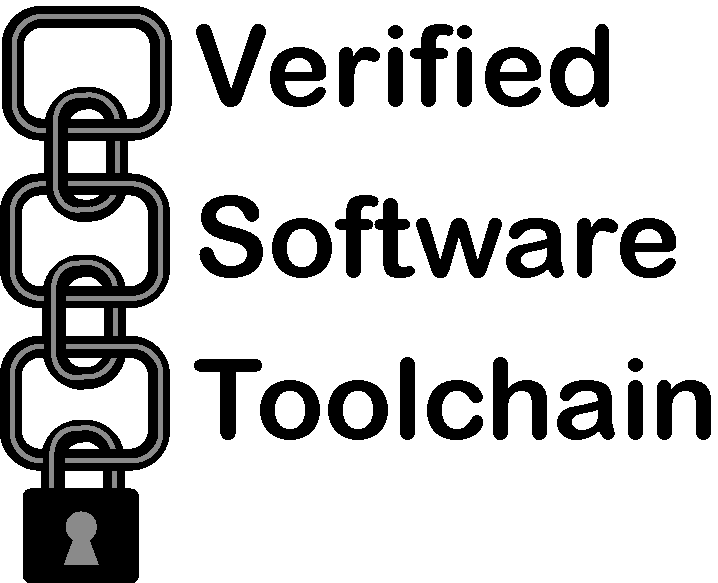
\includegraphics[width=.07\textwidth]{img/chain.png}};


      \draw (0.5,3) node [textstyle, anchor=west, draw=black, thick, minimum width=3cm,minimum height=0.5cm] (ml) {$\Zfield$};
      \draw (0,3) node [anchor=east] (shn) {Mid Level};

      \draw[thick,double, <->, >=implies] (ll.north) -- (ml.south);

      \draw (0.5,4) node [textstyle, anchor=west, draw=black, thick, minimum width=3cm,minimum height=0.5cm] (hl) {$\K$};
      \draw (0,4) node [anchor=east] (shn) {High Level};

      \draw[thick,double, <-, >=implies] (ml.north) -- (hl.south);
    \end{scope}
\end{tikzpicture}

  \caption{Structural construction of the proof}
  \label{tikz:ProofStructure}
\end{figure}





\subsection{A Correct Specification}

TweetNaCl implements X25519 with numbers represented as arrays.
RFC~7748 defines X25519 over field elements. In order to simplify our proofs,
we define operations used in the ladder over generic types
\coqe{T} and \coqe{T'}. Those types are later instantiated as natural numbers,
integers, field elements, list of integers...
The generic definition of the ladder (\coqe{montgomery_rec}) and its match with
the definition of RFC~7748 are provided in Appendix~\ref{subsubsec:coq-ladder}.
It has to be noted that the RFC uses an additional variable to optimize the number
of \texttt{CSWAP}:
\emph{``Note that these formulas are slightly different from Montgomery's
original paper.  Implementations are free to use any correct formulas.''}~\cite{rfc7748}.
We later prove our ladder correct in that respect (\sref{sec:maths}).

\coqe{montgomery_rec} only computes the ladder steps.
While the inversion, the packing, the unpacking (setting bit 255 to \texttt{0})
and the clamping are not defined in a generic manner, we show their equivalence
between the different representations.

Appendix~\ref{subsubsec:ZCryptoScalarmult} shows the instantiation of our ladder
over Integers (type \coqe{Z}). We call it \coqe{ZCrypto_Scalarmult}.
The modulo reduction is applied in \coqe{ZPack25519} translating every
underlying operations as over \Zfield. As a result this specification can be
interpreted as the formalization of X25519 in RFC~7748.

In appendix~\ref{subsubsec:CryptoScalarmult}, we show the the formalization of
\TNaCle{crypto_scalarmult} over lists of integers. We define it as
\Coqe{Crypto_Scalarmult} or \Coqe{CSM}. For the sake of space and simplicity we
do not display the definitions of each underlying functions.
The location of the definitions are listed in Appendix~\ref{appendix:proof-files}.

\subsection{With the Verifiable Software Toolchain}
\label{subsec:with-VST}

We now turn our focus to the specification of the Hoare triple with our
specifications of \TNaCle{crypto_scalarmult} over lists of integers and proving
its correctness.

\subheading{Specifications.}
We show the soundness of TweetNaCl by proving the following specification matches
a pure Coq function.
% why "pure" ?
% A pure function is a function where the return value is only determined by its
% input values, without observable side effects (Side effect are e.g. printing)
This defines the equivalence between the Clight representation and our Coq
definition of the ladder (\coqe{CSM}).

\begin{lstlisting}[language=CoqVST]
Definition crypto_scalarmult_spec :=
DECLARE _crypto_scalarmult_curve25519_tweet
WITH
  v_q: val, v_n: val, v_p: val, c121665:val,
  sh : share,
  q : list val, n : list Z, p : list Z
(*------------------------------------------*)
PRE [ _q OF (tptr tuchar),
     _n OF (tptr tuchar),
     _p OF (tptr tuchar) ]
PROP (writable_share sh;
      Forall (fun x => 0 <= x < 2^8) p;
      Forall (fun x => 0 <= x < 2^8) n;
      Zlength q = 32; Zlength n = 32;
      Zlength p = 32)
LOCAL(temp _q v_q; temp _n v_n; temp _p v_p;
      gvar __121665 c121665)
SEP  (sh [{ v_q }] <<(uch32)-- q;
      sh [{ v_n }] <<(uch32)-- mVI n;
      sh [{ v_p }] <<(uch32)-- mVI p;
      Ews [{ c121665 }] <<(lg16)-- mVI64 c_121665)
(*------------------------------------------*)
POST [ tint ]
PROP (Forall (fun x => 0 <= x < 2^8) (CSM n p);
      Zlength (CSM n p) = 32)
LOCAL(temp ret_temp (Vint Int.zero))
SEP  (sh [{ v_q }] <<(uch32)-- mVI (CSM n p);
      sh [{ v_n }] <<(uch32)-- mVI n;
      sh [{ v_p }] <<(uch32)-- mVI p;
      Ews [{ c121665 }] <<(lg16)-- mVI64 c_121665
\end{lstlisting}

In this specification we state as preconditions:
\begin{itemize}
  \item[] \VSTe{PRE}: \VSTe{_p OF (tptr tuchar)}\\
  The function \TNaCle{crypto_scalarmult} takes as input three pointers to
  arrays of unsigned bytes (\VSTe{tptr tuchar}) \VSTe{_p}, \VSTe{_q} and \VSTe{_n}.
  \item[] \VSTe{LOCAL}: \VSTe{temp _p v_p}\\
  Each pointer represent an address \VSTe{v_p},
  \VSTe{v_q} and \VSTe{v_n}.
  \item[] \VSTe{SEP}: \VSTe{sh [{ v_p $\!\!\}\!\!]\!\!\!$ <<(uch32)-- mVI p}\\
  In the memory share \texttt{sh}, the address \VSTe{v_p} points
  to a list of integer values \VSTe{mVI p}.
  \item[] \VSTe{PROP}: \VSTe{Forall (fun x => 0 <= x < 2^8) p}\\
  In order to consider all the possible inputs, we assumed each
  elements of the list \texttt{p} to be bounded by $0$ included and $2^8$
  excluded.
  \item[] \VSTe{PROP}: \VSTe{Zlength p = 32}\\
  We also assumed that the length of the list \texttt{p} is 32. This defines the
  complete representation of \TNaCle{u8[32]}.
\end{itemize}

As Post-condition we have:
\begin{itemize}
  \item[] \VSTe{POST}: \VSTe{tint}\\
  The function \TNaCle{crypto_scalarmult} returns an integer.
  \item[] \VSTe{LOCAL}: \VSTe{temp ret_temp (Vint Int.zero)}\\
  The returned integer has value $0$.
  \item[] \VSTe{SEP}: \VSTe{sh [{ v_q $\!\!\}\!\!]\!\!\!$ <<(uch32)-- mVI (CSM n p)}\\
  In the memory share \texttt{sh}, the address \VSTe{v_q} points
  to a list of integer values \VSTe{mVI (CSM n p)} where \VSTe{CSM n p} is the
  result of the \VSTe{crypto_scalarmult} over \VSTe{n} and \VSTe{p}.
  \item[] \VSTe{PROP}: \VSTe{Forall (fun x => 0 <= x < 2^8) (CSM n p)}\\
  \VSTe{PROP}: \VSTe{Zlength (CSM n p) = 32}\\
  We show that the computation for \VSTe{CSM} fits in  \TNaCle{u8[32]}.
\end{itemize}

This specification shows that \TNaCle{crypto_scalarmult} in C computes the same
result as \VSTe{CSM} in Coq provided that inputs are within their respective
bounds: arrays of 32 bytes.
The location of the proof of this Hoare triple can be found in Appendix~\ref{appendix:proof-files}.

% We now bring the attention of the reader to details of verifications using the VST.

%% BLABLA about VST. Does not belong here.

% The Verifiable Software Toolchain uses a strongest postcondition strategy.
% The user must first write a formal specification of the function he wants to verify in Coq.
% This should be as close as possible to the C implementation behavior.
% This will simplify the proof and help with stepping through the Clight version of the software.
% With the range of inputs defined, VST mechanically steps through each instruction
% and ask the user to verify auxiliary goals such as array bound access, or absence of overflows/underflows.
% We call this specification a low level specification. A user will then have an easier
% time to prove that his low level specification matches a simpler higher level one.

% In order to further speed-up the verification process, it has to be know that to
% prove the specification \TNaCle{crypto_scalarmult}, a user only need the specification of e.g. \TNaCle{M}.
% This provide with multiple advantages: the verification by the Coq kernel can be done
% in parallel and multiple users can work on proving different functions at the same time.
% For the sake of completeness we proved all intermediate functions.

\subheading{Memory aliasing.}
In the VST, a simple specification of \texttt{M(o,a,b)} will assume three
distinct memory share. When called with three memory shares (\texttt{o, a, b}),
the three of them will be consumed. However assuming this naive specification
when \texttt{M(o,a,a)} is called (squaring), the first two memory shares (\texttt{o, a})
are consumed and VST will expect a third memory share (\texttt{a}) which does not \textit{exist} anymore.
Examples of such cases are illustrated in \fref{tikz:MemSame}.
\begin{figure}[h]
  \centering
  \begin{tikzpicture}
\draw (0,0) rectangle (3,0.3);
\draw[thick] (1,0) -- (1,0.3);
\draw[thick] (2,0) -- (2,0.3);
\node [anchor=east] (shn) at (0,0.15) {sh};
\node [anchor=north] (Moab) at (1.5,-0.5) {\texttt{M(o,a,b)}};
\draw[thick, -> ] (1.25, -0.6) -- (1.25, -0.5) -- (0.5,-0.1);
\draw[thick, -> ] (1.6, -0.6) -- (1.6, -0.5) -- (1.5,-0.1);
\draw[thick, -> ] (1.95, -0.6) -- (1.95, -0.5) -- (2.5,-0.1);

\node [anchor=north west, text width=6cm, align=left] (Sepoab) at (-0.5,-1.8)
  {\VSTess{sh [{ v_o $\!\!\}\!\!]\!\!\!$ <<(lg16)-- o}\\[-0.2em]
  \VSTess{sh [{ v_a $\!\!\}\!\!]\!\!\!$ <<(lg16)-- a}\\[-0.2em]
  \VSTess{sh [{ v_b $\!\!\}\!\!]\!\!\!$ <<(lg16)-- b}};


\begin{scope}[yshift=0 cm,xshift=4.5 cm]
  \draw (0,0) rectangle (2,0.3);
  \draw[thick] (1,0) -- (1,0.3);
  % \draw[thick] (2,0) -- (2,0.3);
  \node [anchor=east] (shm) at (0,0.15) {sh};
  \node [anchor=north] (Mcaa) at (1,-0.5) {\texttt{M(c,c,a)}};
  \draw[thick, -> ] (0.75, -0.6) -- (0.75, -0.5) -- (0.4,-0.1);
  \draw[thick, -> ] (1.1, -0.6) -- (1.1, -0.5) -- (0.6,-0.1);
  \draw[thick, -> ] (1.45, -0.6) -- (1.45, -0.5) -- (1.5,-0.1);

  \node [anchor=north west, text width=6cm, align=left] (Sepoab) at (-0.5,-1.8)
    {\VSTess{sh [{ v_c $\!\!\}\!\!]\!\!\!$ <<(lg16)-- c}\\[-0.2em]
    \VSTess{sh [{ v_a $\!\!\}\!\!]\!\!\!$ <<(lg16)-- a}};
\end{scope}

\draw[dashed] (-0.5,-1.2) -- +(8,0);
\node [anchor=north west] (sep) at (-0.5,-1.2) {In Separation Logic:};

\begin{scope}[yshift=-4.25 cm,xshift=2 cm]
  \draw (0,0) rectangle (2,0.3);
  \draw[thick] (1,0) -- (1,0.3);
  \node [anchor=east] (shm) at (0,0.15) {sh\;};

  \draw (0,0.5) rectangle (1,0.8);
  \node [anchor=east] (shm) at (0,0.65) {Ews};

  \draw[thick] (2,0) -- (2,0.3);
  \node [anchor=north west] (Mcaa) at (0.15,-0.5) {\texttt{M(a,c,\_121665)}};
  \draw[thick, -> ] (0.75, -0.6) -- (0.75, -0.5) -- (0.5,-0.1);
  \draw[thick, -> ] (1.1, -0.6) -- (1.1, -0.5) -- (1.5,-0.1);
  \draw[thick, -> ] (2.0, -0.6) -- (2.45, -0.2) -- (2.45, 0.3) -- (2.2, 0.65) -- (1.5,0.65);

  \node [anchor=north west, text width=6cm, align=left] (Sepoab) at (-0.5,-1.8)
    {\VSTess{sh [{ v_a $\!\!\}\!\!]\!\!\!$ <<(lg16)-- a}\\[-0.2em]
    \VSTess{sh [{ v_c $\!\!\}\!\!]\!\!\!$ <<(lg16)-- c}\\[-0.2em]
    \VSTess{Ews [{ __121665 $\!\!\}\!\!]\!\!\!$ <<(lg16)-- _121665}
    };
\end{scope}
\draw[dashed] (0.5,-5.45) -- +(6,0);
\node [anchor=north west] (sep) at (0.5,-5.45) {In Separation Logic:};
\end{tikzpicture}%

  \caption{Aliasing and Separation Logic}
  \label{tikz:MemSame}
\end{figure}

As a result, a function must either have multiple specifications or specify which
aliasing case is being used.
The first option would require us to do very similar proofs multiple times for a same function.
We chose the second approach: for functions with 3 arguments, named hereafter \texttt{o, a, b},
we define an additional parameter $k$ with values in $\{0,1,2,3\}$:
\begin{itemize}
  \item if $k=0$ then \texttt{o} and \texttt{a} are aliased.
  \item if $k=1$ then \texttt{o} and \texttt{b} are aliased.
  \item if $k=2$ then \texttt{a} and \texttt{b} are aliased.
  \item else there is no aliasing.
\end{itemize}
In the proof of our specification, we do a case analysis over $k$ when needed.
This solution does not cover all cases (e.g. all arguments are aliased) but it
is enough for our needs.

\subheading{Verifying \texttt{for} loops.}
Final state of \texttt{for} loops are usually computed by simple recursive functions.
However we must define invariants which are true for each iteration step.

Assume we want to prove a decreasing loop where indexes go from 3 to 0.
Define a function $g : \N \rightarrow State  \rightarrow State $ which takes as
input an integer for the index and a state, then returns a state.
It simulates the body of the \texttt{for} loop.
Assume its recursive call: $f : \N \rightarrow State \rightarrow State $ which
iteratively applies $g$ with decreasing index:
\begin{equation*}
  f ( i , s ) =
  \begin{cases}
  s & \text{if } s = 0 \\
  f( i - 1 , g ( i - 1  , s )) & \text{otherwise}
  \end{cases}
\end{equation*}
Then we have :
\begin{align*}
  f(4,s) &= g(0,g(1,g(2,g(3,s))))
  % \\
  % f(3,s) &= g(0,g(1,g(2,s)))
\end{align*}
To prove the correctness of $f(4,s)$, we need to prove that intermediate steps
$g(3,s)$; $g(2,g(3,s))$; $g(1,g(2,g(3,s)))$; $g(0,g(1,g(2,g(3,s))))$ are correct.
Due to the computation order of recursive function, our loop invariant for
$i\in\{0;1;2;3;4\}$ cannot use $f(i)$.
To solve this, we define an auxiliary function with an accumulator such that
given $i\in\{0;1;2;3;4\}$, it will compute the first $i$ steps of the loop.

We then prove for the complete number of steps, the function with the accumulator
and without returns the same result.
We formalized this result in a generic way in Appendix~\ref{subsubsec:for}.

Using this formalization, we prove that the 255 steps of the Montgomery ladder
in C provide the same computations as in \coqe{CSM}.




\subsection{Number Representation and C Implementation}

As described in \sref{subsec:Number-TweetNaCl}, numbers in \TNaCle{gf} are represented
in base $2^{16}$ and we use a direct mapping to represent that array as a list
integers in Coq. However in order to show the correctness of the basic operations,
we need to convert this number to a full integer.
\begin{dfn}
Let \Coqe{ZofList} : $\Z \rightarrow \texttt{list} \Z \rightarrow \Z$,
a parameterized map by $n$ between a list $l$ and its little endian representation
with a radix $2^n$.
\end{dfn}
We define it in Coq as:
\begin{lstlisting}[language=Coq]
Fixpoint ZofList {n:Z} (a:list Z) : Z :=
  match a with
  | [] => 0
  | h :: q => h + (pow 2 n) * ZofList q
  end.
\end{lstlisting}
We define a notation where $n$ is $16$.
\begin{lstlisting}[language=Coq]
Notation "Z16.lst A" := (ZofList 16 A).
\end{lstlisting}
To facilitate working in \Zfield, we define the \coqe{:GF} notation.
\begin{lstlisting}[language=Coq]
Notation "A :GF" := (A mod (2^255-19)).
\end{lstlisting}
Later in \sref{sec:maths}, we formally define \F{\p}.
Equivalence between operations under \coqe{:GF} and in \F{\p} are easily proven.

Using these two definitions, we proved intermediates lemmas such as the correctness of the
multiplication \Coqe{Low.MM} where \Coqe{Low.M} replicate the computations and steps done in C.
\begin{lemma}
  \label{lemma:mult_correct}
  \Coqe{Low.M} implements correctly the multiplication over \Zfield.
\end{lemma}
And seen in Coq as follows:
\begin{lstlisting}[language=Coq]
Lemma mult_GF_Zlength :
  forall (a:list Z) (b:list Z),
  Zlength a = 16 ->
  Zlength b = 16 ->
   (Z16.lst (Low.M a b)) :GF =
   (Z16.lst a * Z16.lst b) :GF.
\end{lstlisting}

However for our purpose, simple functional correctness is not enough.
We also need to define the bounds under which the operation is correct,
allowing us to chain them, guaranteeing us the absence of overflow.

\begin{lemma}
  \label{lemma:mult_bounded}
  if all the values of the input arrays are constrained between $-2^{26}$ and $2^{26}$,
  then the output of \coqe{Low.M} will be constrained between $-38$ and $2^{16} + 38$.
\end{lemma}
And seen in Coq as follows:
\begin{lstlisting}[language=Coq]
Lemma M_bound_Zlength :
  forall (a:list Z) (b:list Z),
  Zlength a = 16 ->
  Zlength b = 16 ->
  Forall (fun x => -2^26 < x < 2^26) a ->
  Forall (fun x => -2^26 < x < 2^26) b ->
    Forall (fun x => -38 <= x < 2^16 + 38) (Low.M a b).
\end{lstlisting}




\subsection{Inversions, Reflections and Packing}

We now turn our attention to the inversion in \Zfield and techniques to
increase the verification speed of complex formulas.

\subheading{Inversions in \Zfield.}
We define a Coq version of the inversion mimicking
the behavior of \TNaCle{inv25519} (see below) over \Coqe{list Z}.
\begin{lstlisting}[language=Ctweetnacl]
sv inv25519(gf o,const gf i)
{
  gf c;
  int a;
  set25519(c,i);
  for(a=253;a>=0;a--) {
    S(c,c);
    if(a!=2&&a!=4) M(c,c,i);
  }
  FOR(a,16) o[a]=c[a];
}
\end{lstlisting}
We specify this with 2 functions: a recursive \Coqe{pow_fn_rev}
to simulate the \texttt{for} loop and a simple \Coqe{step_pow} containing the body.
\begin{lstlisting}[language=Coq]
Definition step_pow (a:Z)
  (c:list Z) (g:list Z) : list Z :=
  let c := Sq c in
    if a <>? 2 && a <>? 4
    then M c g
    else c.

Function pow_fn_rev (a:Z) (b:Z)
  (c: list Z) (g: list Z)
  {measure Z.to_nat a} : (list Z) :=
  if a <=? 0
    then c
    else
      let prev := pow_fn_rev (a - 1) b c g in
        step_pow (b - a) prev g.
\end{lstlisting}
This \Coqe{Function} requires a proof of termination. It is done by proving the
well-foundedness of the decreasing argument: \Coqe{measure Z.to_nat a}. Calling
\Coqe{pow_fn_rev} 254 times allows us to reproduce the same behavior as the Clight definition.
\begin{lstlisting}[language=Coq]
Definition Inv25519 (x:list Z) : list Z :=
  pow_fn_rev 254 254 x x.
\end{lstlisting}
Similarly we define the same function over $\Z$.
\begin{lstlisting}[language=Coq]
Definition step_pow_Z (a:Z) (c:Z) (g:Z) : Z :=
  let c := c * c in
  if a <>? 2 && a <>? 4
    then c * g
    else c.

Function pow_fn_rev_Z (a:Z) (b:Z) (c:Z) (g: Z)
  {measure Z.to_nat a} : Z :=
  if (a <=? 0)
    then c
    else
      let prev := pow_fn_rev_Z (a - 1) b c g in
        step_pow_Z (b - a) prev g.

Definition Inv25519_Z (x:Z) : Z :=
  pow_fn_rev_Z 254 254 x x.
\end{lstlisting}
By using \lref{lemma:mult_correct}, we prove their equivalence in $\Zfield$.
\begin{lemma}
\label{lemma:Inv_equivalence}
The function \coqe{Inv25519} over list of integers computes the same
result at \coqe{Inv25519_Z} over integers in \Zfield.
\end{lemma}
This is formalized in Coq as follows:
\begin{lstlisting}[language=Coq]
Lemma Inv25519_Z_GF : forall (g:list Z),
  length g = 16 ->
  (Z16.lst (Inv25519 g)) :GF =
  (Inv25519_Z (Z16.lst g)) :GF.
\end{lstlisting}

In TweetNaCl, \TNaCle{inv25519} computes an inverse in $\Zfield$.
It uses Fermat's little theorem by doing an exponentiation to $2^{255}-21$.
This is done by applying a square-and-multiply algorithm. The binary representation
of $p-2$ implies to always do multiplications except for bits 2 and 4.
To prove the correctness of the result we can use multiple strategies such as:
\begin{itemize}
  \item Proving it is a special case of square-and-multiply algorithm applied to $2^{255}-21$.
  \item Unrolling the for loop step-by-step and applying the equalities
  $x^a \times x^b = x^{(a+b)}$ and $(x^a)^2 = x^{(2 \times a)}$. We prove that
  the resulting exponent is $2^{255}-21$.
\end{itemize}
We use the second method for the benefits of simplicity. However it requires to
apply the unrolling and exponentiation formulas 255 times. This can be automated
in Coq with tacticals such as \Coqe{repeat}, but it generates a proof object which
will take a long time to verify.


\subheading{Speeding up with Reflections.} This technique provides us with
flexibility, \eg we don't need to know the number of times nor the order
in which the lemmas needs to be applied (chapter 15 in \cite{CpdtJFR}).

The idea is to \textit{reflect} the goal into a decidable environment.
We show that for a property $P$, we can define a decidable Boolean property
$P_{bool}$ such that if $P_{bool}$ is \Coqe{true} then $P$ holds.
$$reify\_P : P_{bool} = true \implies P$$
By applying $reify\_P$ on $P$ our goal become $P_{bool} = true$.
We then compute the result of $P_{bool}$. If the decision goes well we are
left with the tautology $true = true$.

To prove that the \Coqe{Inv25519_Z} is computing $x^{2^{255}-21}$,
we define a Domain Specific Language (DSL).
\begin{dfn}
Let \Coqe{expr_inv} denote an expression which is either a term;
a multiplication of expressions; a squaring of an expression or a power of an expression.
And Let \Coqe{formula_inv} denote an equality between two expressions.
\end{dfn}
\begin{lstlisting}[language=Coq]
Inductive expr_inv :=
  | R_inv : expr_inv
  | M_inv : expr_inv -> expr_inv -> expr_inv
  | S_inv : expr_inv -> expr_inv
  | P_inv : expr_inv -> positive -> expr_inv.

Inductive formula_inv :=
  | Eq_inv : expr_inv -> expr_inv -> formula_inv.
\end{lstlisting}
The denote functions are defined as follows:
\begin{lstlisting}[language=Coq]
Fixpoint e_inv_denote (m:expr_inv) : Z :=
  match m with
  | R_inv     =>
    term_denote
  | M_inv x y =>
    (e_inv_denote x) * (e_inv_denote y)
  | S_inv x =>
    (e_inv_denote x) * (e_inv_denote x)
  | P_inv x p =>
    pow (e_inv_denote x) (Z.pos p)
  end.

Definition f_inv_denote (t : formula_inv) : Prop :=
  match t with
  | Eq_inv x y => e_inv_denote x = e_inv_denote y
  end.
\end{lstlisting}
All denote functions also take as an argument the environment containing the variables.
We do not show it here for the sake of readability,
given that an environment, \Coqe{term_denote} returns the appropriate variable.
With this Domain Specific Language we have the following equality:
\begin{lstlisting}[backgroundcolor=\color{white}]
f_inv_denote
 (Eq_inv (M_inv R_inv (S_inv R_inv))
         (P_inv R_inv 3))
  = (x * x^2 = x^3)
\end{lstlisting}
On the right side, \Coqe{(x * x^2 = x^3)} depends on $x$. On the left side,
\texttt{(Eq\_inv (M\_inv R\_inv (S\_inv R\_inv)) (P\_inv R\_inv 3))} does not depend on $x$.
This allows us to use computations in our decision procedure.

We define \Coqe{step_inv} and \Coqe{pow_inv} to mirror the behavior of
\Coqe{step_pow_Z} and respectively \Coqe{pow_fn_rev_Z} over our DSL and
we prove their equality.
\begin{lstlisting}[language=Coq]
Lemma step_inv_step_pow_eq :
  forall (a:Z) (c:expr_inv) (g:expr_inv),
  e_inv_denote (step_inv a c g) =
  step_pow_Z a (e_inv_denote c) (e_inv_denote g).

Lemma pow_inv_pow_fn_rev_eq :
  forall (a:Z) (b:Z) (c:expr_inv) (g:expr_inv),
  e_inv_denote (pow_inv a b c g) =
  pow_fn_rev_Z a b (e_inv_denote c) (e_inv_denote g).
\end{lstlisting}
We then derive the following lemma.
\begin{lemma}
\label{lemma:reify}
With an appropriate choice of variables, \Coqe{pow_inv} denotes \Coqe{Inv25519_Z}.
\end{lemma}

In order to prove formulas in \Coqe{formula_inv},
we have the following a decidable procedure.
We define \Coqe{pow_expr_inv}, a function which returns the power of an expression.
We then compare the two values and decide over their equality.
\begin{lstlisting}[language=Coq]
Fixpoint pow_expr_inv (t:expr_inv) : Z :=
  match t with
  (* power of a term is 1. *)
  | R_inv   => 1
  (* x^a * x^b = x^{a+b}. *)
  | M_inv x y =>
    (pow_expr_inv x) + (pow_expr_inv y)
    (* (x^a)^2 = x^{2a}. *)
  | S_inv x =>
    2 * (pow_expr_inv x)
    (* (x^b)^a = x^{a*b}. *)
  | P_inv x p =>
    (Z.pos p) * (pow_expr_inv x)
  end.

Definition decide_e_inv (l1 l2:expr_inv) : bool :=
  (pow_expr_inv l1) ==? (pow_expr_inv l2).

Definition decide_f_inv (f:formula_inv) : bool :=
  match f with
  | Eq_inv x y => decide_e_inv x y
  end.
\end{lstlisting}

We prove our decision procedure correct.
\begin{lemma}
\label{lemma:decide}
For all formulas $f$, if the decision over $f$ returns \Coqe{true},
then the denoted equality by $f$ is true.
\end{lemma}
Which is formalized as:
\begin{lstlisting}[language=Coq]
Lemma decide_formula_inv_impl :
  forall (f:formula_inv),
  decide_f_inv f = true ->
    f_inv_denote f.
\end{lstlisting}

By reification to over DSL (\lref{lemma:reify}) and by applying our decision
(\lref{lemma:decide}), we prove the following corollary.
\begin{lemma}
\label{lemma:inv_comput_inv}
\Coqe{Inv25519_Z} computes an inverse in \Zfield.
\end{lemma}
Which is formalized as:
\begin{lstlisting}[language=Coq]
Theorem Inv25519_Z_correct :
  forall (x:Z),
  Inv25519_Z x = pow x (2^255-21).
\end{lstlisting}

% From \Coqe{Inv25519_Z_GF} (\lref{lemma:Inv_equivalence}) and \Coqe{Inv25519_Z_correct} (Corollary~\ref{lemma:inv_comput_inv}),
From \lref{lemma:Inv_equivalence} and Corollary~\ref{lemma:inv_comput_inv},
we conclude the functional correctness of the inversion over \Zfield.
\begin{corollary}
\label{cor:inv_comput_field}
\Coqe{Inv25519} computes an inverse in \Zfield.
\end{corollary}
Which is formalized as:
\begin{lstlisting}[language=Coq]
Corollary Inv25519_Zpow_GF :
  forall (g:list Z),
  length g = 16 ->
  Z16.lst (Inv25519 g) :GF  =
  (pow (Z16.lst g) (2^255-21)) :GF.
\end{lstlisting}

\subheading{Another applications of reflections: packing}
This reflection technique can also be used where proofs requires some computing
over a small and finite domain of variables to test e.g. for all $i$ such that $0 \le i < 16$.
Using reflection we prove that we can split the for loop in \TNaCle{pack25519} into two parts.
\begin{lstlisting}[language=Ctweetnacl]
for(i=1;i<15;i++) {
  m[i]=t[i]-0xffff-((m[i-1]>>16)&1);
  m[i-1]&=0xffff;
}
\end{lstlisting}
The first loop is computing the subtraction while the second is applying the carries.
\begin{lstlisting}[language=Ctweetnacl]
for(i=1;i<15;i++) {
  m[i]=t[i]-0xffff
}

for(i=1;i<15;i++) {
  m[i]=m[i]-((m[i-1]>>16)&1);
  m[i-1]&=0xffff;
}
\end{lstlisting}

This loop separation allows simpler proofs. The first loop is seen as the subtraction of a number in \Zfield.
We then prove that with the iteration of the second loop, the number represented in $\Zfield$ stays the same.
This leads to the proof that \TNaCle{pack25519} is effectively reducing modulo $\p$ and returning a number in base $2^8$.
\begin{lstlisting}[language=Coq]
Lemma Pack25519_mod_25519 :
  forall (l:list Z),
  Zlength l = 16 ->
  Forall (fun x => -2^62 < x < 2^62) l ->
  ZofList 8 (Pack25519 l) =
  (Z16.lst l) mod (2^255-19).
\end{lstlisting}

By proving that each functions \coqe{Low.M}; \coqe{Low.A}; \coqe{Low.Sq}; \coqe{Low.Zub};
\coqe{Unpack25519}; \coqe{clamp}; \coqe{Pack25519}; \coqe{car25519} are behaving over \coqe{list Z}
as their equivalent over \coqe{Z} in \coqe{:GF} (in \Zfield), we prove the correctness of
\tref{thm:RFC}. This is formalized as follows in Coq:
\begin{lstlisting}[language=Coq]
Theorem Crypto_Scalarmult_Eq :
  forall (n p:list Z),
  Zlength n = 32 ->
  Zlength p = 32 ->
  Forall (fun x : Z, 0 <= x /\ x < 2 ^ 8) n ->
  Forall (fun x : Z, 0 <= x /\ x < 2 ^ 8) p ->
  ZofList 8 (Crypto_Scalarmult n p) =
  ZCrypto_Scalarmult (ZofList 8 n) (ZofList 8 p).
\end{lstlisting}

\section{Proving that X25519 in Coq matches the mathematical model}
\label{sec3-maths}

In this section we first present the work of Bartzia and Strub \cite{DBLP:conf/itp/BartziaS14} (\ref{Weierstrass}).
We extend it to support Montgomery curves (\ref{montgomery}) with homogeneous coordinates (\ref{projective}) and prove the correctness of the ladder (\ref{ladder}).

We then prove the montgomery ladder computes
the x-coordinate of scalar multiplication over $\F{p^2}$
(Theorem 2.1 by Bernstein \cite{Ber06}) where $p$ is the prime $\p$.

\subsection{Formalization of Elliptic Curves}

We consider elliptic curves over a field $\K$. We assume that the
characteristic of $\K$ is neither 2 or 3.

\begin{definition}
Let a field $\K$, using an appropriate choice of coordinates, an elliptic curve $E$
is a plane cubic albreaic curve $E(x,y)$ defined by an equation of the form:
$$E : y^2 + a_1 xy + a_3 y = x^3 + a_2 x^2 + a_4 x + a_6$$
where the $a_i$'s are in \K\ and the curve has no singular point (\ie no cusps
or self-intersections). The set of points, written $E(\K)$, is formed by the
solutions $(x,y)$ of $E$ augmented by a distinguished point $\Oinf$ (called point at infinity):
$$E(\K) = \{(x,y) \in \K \times \K | E(x,y)\} \cup \{\Oinf\}$$
\end{definition}

\subsubsection{Weierstra{\ss} Curves}
\label{Weierstrass}
This equation $E(x,y)$ can be reduced into its Weierstra{\ss} form.

\begin{definition}
Let $a \in \K$, and $b \in \K$ such that $$\Delta(a,b) = -16(4a^3 + 27b^2) \neq 0.$$ The \textit{elliptic curve} $E_{a,b}(\K)$ is the set of all points $(x,y) \in \K^2$ satisfying the equation:
$$y^2 = x^3 + ax + b,$$
along with an additional formal point $\Oinf$, ``at infinity''. Such curve does not present any singularity.
\end{definition}

In this setting, Bartzia and Strub defined the parametric type \texttt{ec} which
represent the points on a specific curve. It is parametrized by
a \texttt{K : ecuFieldType} -- the type of fields which characteristic is not 2 or 3 --
and \texttt{E : ecuType} -- a record that packs the curve parameters $a$ and $b$
along with the proof that $\Delta(a,b) \neq 0$.
\begin{lstlisting}[language=Coq]
Inductive point := EC_Inf | EC_In of K * K.
Notation "(| x, y |)" := (EC_In x y).
Notation "\infty" := (EC_Inf).

Record ecuType :=
  { A : K; B : K; _ : 4 * A^3 + 27 * B^2 != 0}.
Definition oncurve (p : point) :=
  if p is (| x, y |)
    then y^2 == x^3 + A * x + B
    else true.
Inductive ec : Type := EC p of oncurve p.
\end{lstlisting}

Points of an elliptic curve can be equiped with a structure of an abelian group.
\begin{itemize}
  \item The negation of a point $P = (x,y)$ by taking the symetric with respect to the x axis $-P = (x, -y)$.
  \item The addition of two points $P$ and $Q$ is defined by the negation of third intersection
  of the line passing by $P$ and $Q$ or tangent to $P$ if $P = Q$.
  \item $\Oinf$ is the neutral element under this law: if 3 points are colinear, their sum is equal to $\Oinf$.
\end{itemize}

This operaction are defined in Coq as follow:
\begin{lstlisting}[language=Coq]
Definition neg (p : point) :=
  if p is (| x, y |) then (| x, -y |) else EC_Inf.

Definition add (p1 p2 : point) :=
  match p1, p2 with
    | \infty , _ => p2
    | _ , \infty => p1
    | (| x1, y1 |), (| x2, y2 |) =>
      if x1 == x2 then ... else
        let s := (y2 - y1) / (x2 - x1) in
        let xs := s^2 - x1 - x2 in
          (| xs, - s * (xs - x1 ) - y1 |)
  end.
\end{lstlisting}

And is proven internal to the curve (with coercion):
\begin{lstlisting}[language=Coq]
Lemma addO (p q : ec): oncurve (add p q).

Definition addec (p1 p2 : ec) : ec :=
  EC p1 p2 (addO p1 p2)
\end{lstlisting}

\subsubsection{Montgomery Curves}
\label{montgomery}
Computation over elliptic curves are hard. Speedups can be obtained by using
homogeneous coordinates and other forms than the Weierstra{\ss} form. We consider
the Montgomery form \cite{MontgomerySpeeding}.

\begin{definition}
  Let $a \in \K \backslash \{-2, 2\}$, and $b \in \K \backslash \{ 0\}$. The \textit{Montgomery curve} $M_{a,b}(\K)$ is the set of all points $(x,y) \in \K^2$ satisfying the equation:
  $$by^2 = x^3 + ax^2 + x,$$
  along with an additional formal point $\Oinf$, ``at infinity''.
\end{definition}
Using a similar representation, we defined the parametric type \texttt{mc} which
represent the points on a specific montgomery curve. It is parametrized by
a \texttt{K : ecuFieldType} -- the type of fields which characteristic is not 2 or 3 --
and \texttt{M : mcuType} -- a record that packs the curve paramaters $a$ and $b$
along with the proofs that $b \neq 0$ and $a^2 != 4$.
\begin{lstlisting}[language=Coq]
Record mcuType :=
  { cA : K; cB : K; _ : cB != 0; _ : cA^2 != 4}.
Definition oncurve (p : point K) :=
if p is (| x, y |)
  then cB * y^+2 == x^+3 + cA * x^+2 + x
  else true.
Inductive mc : Type := MC p of oncurve p.

Lemma oncurve_mc: forall p : mc, oncurve p.
\end{lstlisting}
We define the addition on Montgomery curves the same way as it it is in the Weierstra{\ss} form,
however the actual computations will be slightly different.
\begin{lstlisting}[language=Coq]
Definition add (p1 p2 : point K) :=
  match p1, p2 with
    | \infty, _ => p2
    | _, \infty => p1
    | (|x1, y1|), (|x2, y2|) =>
      if   x1 == x2
      then if  (y1 == y2) && (y1 != 0)
           then ... else \infty
      else
        let s  := (y2 - y1) / (x2 - x1) in
        let xs := s^+2 * cB - cA - x1 - x2 in
          (| xs, - s * (xs - x1) - y1 |)
    end.
\end{lstlisting}
But we prove it is internal to the curve (again with coercion):
\begin{lstlisting}[language=Coq]
Lemma addO (p q : mc) : oncurve (add p q).
Definition addmc (p1 p2 : mc) : mc :=
  MC p1 p2 (addO p1 p2)
\end{lstlisting}

We then prove a bijection between a Montgomery curve and its Weierstra{\ss} equation.
\begin{lemma}
  Let $M_{a,b}(\K)$ be a Montgomery curve, define $$a' = \frac{3-a^2}{3b^2} \text{\ \ \ \ and\ \ \ \ } b' = \frac{2a^3 - 9a}{27b^3}.$$
  then $E_{a',b'}(\K)$ is an elliptic curve, and the mapping $\varphi : M_{a,b}(\K) \mapsto E_{a',b'}(\K)$ defined as:
  \begin{align*}
    \varphi(\Oinf_M) &= \Oinf_E\\
    \varphi( (x , y) ) &= ( \frac{x}{b} + \frac{a}{3b} , \frac{y}{b} )
  \end{align*}
  is an isomorphism between groups.
\end{lemma}
\begin{lstlisting}[language=Coq]
Definition ec_of_mc_point p :=
  match p with
  | \infty => \infty
  | (|x, y|) => (|x/(M#b) + (M#a)/(3%:R * (M#b)), y/(M#b)|)
  end.
Lemma ec_of_mc_point_ok p :
  oncurve M p ->
  ec.oncurve E (ec_of_mc_point p).

Definition ec_of_mc p :=
  EC (ec_of_mc_point_ok (oncurve_mc p)).

Lemma ec_of_mc_bij : bijective ec_of_mc.
\end{lstlisting}

\subsubsection{Projective Coordinates}
\label{projective}
Points on a projective plane are represented with a triple $(X:Y:Z)$. Any points except $(0:0:0)$ defines a point on a projective plane. A scalar multiple of a point defines the same point, \ie
for all $\alpha \neq 0$, $(X:Y:Z)$ and $(\alpha X:\alpha Y:\alpha Z)$ defines the same point. For $Z\neq 0$, the projective point $(X:Y:Z)$ corresponds to the point $(X/Z,Y/Z)$ on the Euclidian plane, likewise the point $(X,Y)$ on the Euclidian plane corresponds to $(X:Y:1)$ on the projective plane.

We write the equation for a Montgomery curve $M_{a,b}(\K)$ as such:
\begin{equation}
b \bigg(\frac{Y}{Z}\bigg)^2 = \bigg(\frac{X}{Z}\bigg)^3 + a \bigg(\frac{X}{Z}\bigg)^2 + \bigg(\frac{X}{Z}\bigg)
\end{equation}
Multiplying both sides by $Z^3$ yields:
\begin{equation}
b Y^2Z = X^3 + a X^2Z + XZ^2
\end{equation}
With this equation we can additionally represent the ``point at infinity''. By setting $Z=0$, we derive $X=0$, giving us the ``infinite points'' $(0:Y:0)$ with $Y\neq 0$.

By restristing the parameter $a$ of $M_{a,b}(\K)$ such that $a^2-4$ is not a square in \K, we ensure that $(0,0)$ is the only point with a $y$-coordinate of $0$.
\begin{lstlisting}[language=Coq]
Hypothesis mcu_no_square : forall x : K, x^+2 != (M#a)^+2 - 4%:R.
\end{lstlisting}

With those coordinates we prove the following lemmas for the addition of two points.
\begin{definition}Define the functions $\chi$ and $\chi_0$:\\
-- $\chi : M_{a,b}(\K) \to \K \cup \{\infty\}$\\
  such that $\chi(\Oinf) = \infty$ and $\chi((x,y)) = x$.\\
-- $\chi_0 : M_{a,b}(\K) \to \K$\\
  such that $\chi_0(\Oinf) = 0$ and $\chi_0((x,y)) = x$.
\end{definition}
\begin{lemma}
\label{lemma-add}
Let $M_{a,b}(\K)$ be a Montgomery curve such that $a^2-4$ is not a square, and let $X_1, Z_1, X_2, Z_2, X_3, Z_3 \in \K$, such that $(X_1,Z_1) \neq (0,0)$, $(X_2,Z_2) \neq (0,0)$, $X_4 \neq 0$ and $Z_4 \neq 0$.
Define
\begin{align*}
X_3 &= Z_4((X_1 - Z_1)(X_2+Z_2) + (X_1+Z_1)(X_2-Z_2))^2\\
Z_3 &= X_4((X_1 - Z_1)(X_2+Z_2) - (X_1+Z_1)(X_2-Z_2))^2,
\end{align*}
then for any point $P_1$ and $P_2$ on $M_{a,b}(\K)$ such that $X_1/Z_1 = \chi(P_1), X_2/Z_2 = \chi(P_2)$, and $X_4/Z_4 = \chi(P_1 - P_2)$, we have $X_3/Z_3 = \chi(P_1+P_2)$.\\
\textbf{Remark:} For any $x \in \K \backslash\{0\}, x/0$ should be understood as $\infty$.
\end{lemma}
% This can be formalized as follow:
% \begin{lstlisting}[language=Coq]
% Inductive K_infty :=
% | K_Inf : K_infty
% | K_Fin : K -> K_infty.
%
% Definition point_x (p : point K) :=
%   if p is (|x, _|) then K_Fin x else K_Inf.
% Local Notation "p '#x'" := (point_x p) (at level 30).
% Definition point_x0 (p : point K) :=
%   if p is (|x, _|) then x else 0.
%   Local Notation "p '#x0'" := (point_x0 p) (at level 30).
%
% Definition inf_div (x z : K) :=
%   if z == 0 then K_Inf else K_Fin (x / z).
% Definition hom_ok (x z : K) := (x != 0) || (z != 0).
% Lemma montgomery_hom_neq :
%   forall x1 x2 x4 z1 z2 z4 : K,
%   hom_ok x1 z1 -> hom_ok x2 z2 ->
%   (x4 != 0) && (z4 != 0) ->
%   let x3 := z4 * ((x1 - z1)*(x2 + z2)
%     + (x1 + z1)*(x2 - z2))^+2 in
%   let z3 := x4 * ((x1 - z1)*(x2 + z2)
%     - (x1 + z1)*(x2 - z2))^+2 in
%   forall p1 p2 : point K,
%   oncurve M p1 -> oncurve M p2 ->
%   p1#x = inf_div x1 z1 ->
%   p2#x = inf_div x2 z2 ->
%   (p1 \- p2)#x = inf_div x4 z4 ->
%   hom_ok x3 z3 && ((p1 \+ p2)#x == inf_div x3 z3).
% \end{lstlisting}

With those coordinates we also prove a similar lemma for point doubling.
\begin{lemma}
\label{lemma-double}
Let $M_{a,b}(\K)$ be a Montgomery curve such that $a^2-4$ is not a square, and let $X_1, Z_1, X_2, Z_2, X_3, Z_3 \in \K$, such that $(X_1,Z_1) \neq (0,0)$. Define
\begin{align*}
  c &= (X_1 + Z_1)^2 - (X_1 - Z_1)^2\\
X_3 &= (X_1 + Z_1)^2(X_1-Z_1)^2\\
Z_3 &= c\Big((X_1 + Z_1)^2+\frac{a-2}{4}\times c\Big),
\end{align*}
then for any point $P_1$ on $M_{a,b}(\K)$ such that $X_1/Z_1 = \chi(P_1)$, we have $X_3/Z_3 = \chi(2P_1)$.
\end{lemma}
% Which is formalized as follow:
% \begin{lstlisting}[language=Coq]
% Lemma montgomery_hom_eq :
%   forall x1 z1 : K,
%   hom_ok x1 z1 ->
%   let c := (x1 + z1)^+2 - (x1 - z1)^+2 in
%   let x3 := (x1 + z1)^+2 * (x1 - z1)^+2 in
%   let z3 := c * ((x1 + z1)^+2 + (((M#a) - 2%:R)/4%:R) * c) in
%   forall p : point K, oncurve M p ->
%   p#x = inf_div x1 z1 ->
%   (p \+ p)#x = inf_div x3 z3.
% \end{lstlisting}

With these two lemmas (\ref{lemma-add} and \ref{lemma-double}), we have the basic tools to compute efficiently additions and point doubling on projective coordinates.

\subsubsection{Scalar Multiplication Algorithms}
\label{ladder}

Suppose we have a scalar $n$ and a point $P$ on some curve. The most straightforward way to compute $nP$ is to repetitively add $P$ \ie computing $P + \ldots + P$.
However there is an more efficient algorithm which makes use of the binary representation of $n$ and by combining doubling and adding and starting from $\Oinf$.
\eg for $n=11$, we compute $2(2(2(2\Oinf + P)) + P)+ P$.

\begin{algorithm}
\caption{Double-and-add for scalar mult.}
\label{double-add}
\begin{algorithmic}
\REQUIRE{Point $P$, scalars $n$ and $m$, $n < 2^m$}
\ENSURE{$Q = nP$}
\STATE $Q \leftarrow \Oinf$
\FOR{$k$ := $m$ downto $1$}
  \STATE $Q \leftarrow 2Q$
  \IF{$k^{\text{th}}$ bit of $n$ is $1$}
    \STATE $Q \leftarrow Q + P$
  \ENDIF
\ENDFOR
\end{algorithmic}
\end{algorithm}

\begin{lemma}
\label{lemma-double-add}
Algorithm \ref{double-add} is correct, \ie it respects its output conditions given the input conditions.
\end{lemma}

We prove Lemma \ref{lemma-double-add}. However with careful timing, an attacker could reconstruct $n$.
In the case of Curve25519, $n$ is the private key. With the Montgomery's ladder, while it provides slightly more computations and an extra variable, we can prevent the previous weakness.
See Algorithm \ref{montgomery-ladder}.

\begin{algorithm}
\caption{Montgomery ladder for scalar mult.}
\label{montgomery-ladder}
\begin{algorithmic}
\REQUIRE{Point $P$, scalars $n$ and $m$, $n < 2^m$}
\ENSURE{$Q = nP$}
\STATE $Q \leftarrow \Oinf$
\STATE $R \leftarrow P$
\FOR{$k$ := $m$ downto $1$}
  \IF{$k^{\text{th}}$ bit of $n$ is $0$}
    \STATE $R \leftarrow Q + R$
    \STATE $Q \leftarrow 2Q$
  \ELSE
    \STATE $Q \leftarrow Q + R$
    \STATE $R \leftarrow 2R$
  \ENDIF
\ENDFOR
\end{algorithmic}
\end{algorithm}

\begin{lemma}
\label{lemma-montgomery-ladder}
Algorithm \ref{montgomery-ladder} is correct, \ie it respects its output conditions given the input conditions.
\end{lemma}

In Curve25519 we are only interested in the $x$ coordinate of points, using Lemmas \ref{lemma-add} and \ref{lemma-double}, and replacing the if statements with conditional swapping we can define a ladder similar to the one used in TweetNaCl. See Algorithm \ref{montgomery-double-add}

\begin{algorithm}
\caption{Montgomery ladder for scalar multiplication on $M_{a,b}(\K)$ with optimizations}
\label{montgomery-double-add}
\begin{algorithmic}
\REQUIRE{$x \in \K\backslash \{0\}$, scalars $n$ and $m$, $n < 2^m$}
\ENSURE{$a/c = \chi_0(nP)$ for any $P$ such that $\chi_0(P) = x$}
\STATE $(a,b,c,d) \leftarrow (1,x,0,1)$
\FOR{$k$ := $m$ downto $1$}
  \IF{$k^{\text{th}}$ bit of $n$ is $1$}
    \STATE $(a,b) \leftarrow (b,a)$
    \STATE $(c,d) \leftarrow (d,c)$
  \ENDIF
  \STATE $e \leftarrow a + c$
  \STATE $a \leftarrow a - c$
  \STATE $c \leftarrow b + d$
  \STATE $b \leftarrow b - d$
  \STATE $d \leftarrow e^2$
  \STATE $f \leftarrow a^2$
  \STATE $a \leftarrow c \times a$
  \STATE $c \leftarrow b \times e$
  \STATE $e \leftarrow a + c$
  \STATE $a \leftarrow a - c$
  \STATE $b \leftarrow a^2$
  \STATE $c \leftarrow d-f$
  \STATE $a \leftarrow c\times\frac{A - 2}{4}$
  \STATE $a \leftarrow a + d$
  \STATE $c \leftarrow c \times a$
  \STATE $a \leftarrow d \times f$
  \STATE $d \leftarrow b \times x$
  \STATE $b \leftarrow e^2$
  \IF{$k^{\text{th}}$ bit of $n$ is $1$}
    \STATE $(a,b) \leftarrow (b,a)$
    \STATE $(c,d) \leftarrow (d,c)$
  \ENDIF
\ENDFOR
\end{algorithmic}
\end{algorithm}

\begin{lemma}
\label{lemma-montgomery-double-add}
Algorithm \ref{montgomery-double-add} is correct, \ie it respects its output conditions given the input conditions.
\end{lemma}

%% here we have \chi and \chi_0 ...

We formalized this lemma (\ref{lemma-montgomery-double-add}):
\begin{lstlisting}[language=Coq]
Lemma opt_montgomery_x :
  forall (n m : nat) (x : K),
  n < 2^m -> x != 0 ->
  forall (p : mc M), p#x0 = x ->
  opt_montgomery n m x = (p *+ n)#x0.
\end{lstlisting}

We can remark that for an input $x = 0$, the ladder returns $0$.
\begin{lstlisting}[language=Coq]
Lemma opt_montgomery_0:
  forall (n m : nat), opt_montgomery n m 0 = 0.
\end{lstlisting}
Also \Oinf\ is the neutral element over $M_{a,b}(\K)$, we have:
$$\forall P, P + \Oinf\ = P$$
thus we derive the following lemma.
% \begin{lemma}
% \label{lemma-montgomery-double-add}
% Algorithm \ref{montgomery-double-add} is correct even if $x=0$, \ie it respects its output conditions given the input conditions or $x=0$.
% \end{lemma}
\begin{lstlisting}[language=Coq]
Lemma p_x0_0_eq_0 : forall (n : nat) (p : mc M),
  p #x0 = 0%:R -> (p *+ n) #x0 = 0%R.
\end{lstlisting}
And thus the theorem of the correctness of the Montgomery ladder.
\begin{theorem}
\label{montgomery-ladder-correct}
For all $n, m \in \N$, $x \in \K$, $P \in M_{a,b}(\K)$,
if $\chi_0(P) = x$ then Algorithm \ref{montgomery-double-add} returns $\chi_0(nP)$
\end{theorem}
\begin{lstlisting}[language=Coq]
Theorem opt_montgomery_ok (n m: nat) (x : K) :
  n < 2^m ->
  forall (p : mc M), p#x0 = x ->
  opt_montgomery n m x = (p *+ n)#x0.
\end{lstlisting}

\subsection{Curves, Twists and Extension Fields}

One hypothesis to be able to use the above theorem is that $a^2-4$ is not a square:
$$\forall x \in \K,\ x^2 \neq a^2-4$$
As Curve25519 is defined over the field $\K = \F{p^2}$, there exists $x$ such that $x^2 = a^2-4$.
We first study Curve25519 and one of the quadratic twist Twist25519, first defined over \F{p}.

\subsubsection{Curves and Twists}

We define $\F{p}$ as the numbers between $0$ and $p = \p$.
We create a \coqe{Zmodp} module to encapsulate those definitions.
\begin{lstlisting}[language=Coq]
Module Zmodp.
Definition betweenb x y z := (x <=? z) && (z <? y).
Definition p := locked (2^255 - 19).
Fact Hp_gt0 : p > 0.
Inductive type := Zmodp x of betweenb 0 p x.

Lemma Z_mod_betweenb (x y : Z) :
  y > 0 -> betweenb 0 y (x mod y).

Definition pi (x : Z) : type :=
  Zmodp (Z_mod_betweenb x Hp_gt0).
Coercion repr (x : type) : Z :=
  let: @Zmodp x _ := x in x.
End Zmodp.
\end{lstlisting}

We define the basic operations ($+, -, \times$) with their respective neutral elements ($0, 1$).
\begin{lemma}
$\F{p}$ is a commutative ring.
\end{lemma}
% \begin{lstlisting}[language=Coq]
% Definition zero : type := pi 0.
% Definition one : type := pi 1.
% Definition opp (x : type) : type := pi (p - x).
% Definition add (x y : type) : type := pi (x + y).
% Definition sub (x y : type) : type := pi (x - y).
% Definition mul (x y : type) : type := pi (x * y).
%
% Lemma Zmodp_ring :
%   ring_theory zero one add mul sub opp eq.
% \end{lstlisting}
And finally for $a = 486662$, by using the Legendre symbol we prove that $a^2 - 4$ and $2$ are not squares in $\F{p}$.
\begin{lstlisting}[language=Coq]
Lemma a_not_square : forall x: Zmodp.type,
  x^+2 != (Zmodp.pi 486662)^+2 - 4%:R.
\end{lstlisting}
\begin{lstlisting}[language=Coq,label=two_not_square]
Lemma two_not_square : forall x : Zmodp.type,
  x^+2 != 2%:R.
\end{lstlisting}
We consider $M_{486662,1}(\F{p})$ and $M_{486662,2}(\F{p})$, one of its quadratic twist.
% $M_{486662,1}(\F{p})$ has the same equation as $M_{486662,1}(\F{p^2})$ while $M_{486662,2}(\F{p})$ is one of its quadratic twist.


By instanciating theorem \ref{montgomery-ladder-correct} we derive the following two lemmas:
\begin{lemma} For all $x \in \F{p},\ n \in \N,\ P \in \F{p} \times \F{p}$,\\
such that $P \in M_{486662,1}(\F{p})$ and $\chi_0(P) = x$.
Given $n$ and $x$, $Curve25519\_Fp(n,x) = \chi_0(nP)$.
\end{lemma}
\begin{lemma} For all $x \in \F{p},\ n \in \N,\ P \in \F{p} \times \F{p}$\\
such that $P \in M_{486662,2}(\F{p})$ and $\chi_0(P) = x$.
Given $n$ and $x$, $Twist25519\_Fp(n,x) = \chi_0(nP)$.
\end{lemma}
As the Montgomery ladder defined above does not depends on $b$, it is trivial to see that the computations done for points of $M_{486662,1}(\F{p})$ and of $M_{486662,2}(\F{p})$ are the same.
\begin{lstlisting}[language=Coq]
Theorem curve_twist_eq: forall n x,
  curve25519_Fp_ladder n x = twist25519_Fp_ladder n x.
\end{lstlisting}

Because $2$ is not a square in $\F{p}$, it allows us split $\F{p}$ into two sets.
\begin{lemma}
\label{square-or-2square}
For all $x$ in $\F{p}$, there exists $y$ in $\F{p}$ such that
$$y^2 = x\ \ \ \lor\ \ 2y^2 = x$$
\end{lemma}
For all $x \in \F{p}$, we can compute $x^3 + ax^2 + x$. Using Lemma \ref{square-or-2square} we can find a $y$ such that $(x,y)$ is either on the curve or on the quadratic twist:
\begin{lemma}
\label{curve-or-twist}
For all $x \in \F{p}$, there exists a point $P$ over $M_{486662,1}(\F{p})$ or over $M_{486662,2}(\F{p})$ such that the $x$-coordinate of $P$ is $x$.
\end{lemma}
\begin{lstlisting}[language=Coq]
Theorem x_is_on_curve_or_twist: forall x : Zmodp.type,
  (exists (p : mc curve25519_mcuType), p#x0 = x) \/
  (exists (p' : mc twist25519_mcuType), p'#x0 = x).
\end{lstlisting}

\subsubsection{Curve25519 over \F{p^2}}

We use the same definitions as in \cite{Ber06}. We consider the extension field $\F{p^2}$ as the set $\F{p} \times \F{p}$ with $\delta = 2$, in other words,
the polynomial with coefficients in $\F{p}$ modulo $X^2 - 2$. In a similar way as for $\F{p}$ we use Module in Coq.
\begin{lstlisting}[language=Coq]
Module Zmodp.
Inductive type :=
  Zmodp2 (x: Zmodp.type) (y:Zmodp.type).

Definition pi (x : Zmodp.type * Zmodp.type) : type :=
  Zmodp2 x.1 x.2.
Coercion repr (x : type) : Zmodp.type*Zmodp.type :=
  let: Zmodp2 u v := x in (u, v).

Definition zero : type :=
  pi ( 0%:R, 0%:R ).
Definition one : type :=
  pi ( 1, 0%:R ).
Definition opp (x : type) : type :=
  pi (- x.1 , - x.2).
Definition add (x y : type) : type :=
  pi (x.1 + y.1, x.2 + y.2).
Definition sub (x y : type) : type :=
  pi (x.1 - y.1, x.2 - y.2).
Definition mul (x y : type) : type :=
  pi ((x.1 * y.1) + (2%:R * (x.2 * y.2)),
      (x.1 * y.2) + (x.2 * y.1)).
\end{lstlisting}
We define the basic operations ($+, -, \times$) with their respective neutral elements ($0, 1$).
Additionally we verify that for each element of in $\F{p^2}\backslash\{0\}$, there exists a multiplicative inverse.
\begin{lemma} For all $x \in \F{p^2}\backslash\{0\}$ and $a,b \in \F{p}$ such that $x = (a,b)$,
$$x^{-1} = \Big(\frac{a}{a^2-2b^2}\ , \frac{-b}{a^2-2b^2}\Big)$$
\end{lemma}
Similarily as in $\F{p}$, we define $0^{-1} = 0$.
\begin{lemma}
$\F{p^2}$ is a commutative ring.
\end{lemma}
We can then specialize the basic operations in order to speed up the verifications of formulas by using rewrite rules:
\begin{align*}
(a,0) + (b,0) &= (a+b, 0)\\
(a,0) \cdot   (b,0) &= (a \cdot b, 0)\\
(a, 0)^n &= (a^n, 0)\\
(a, 0)^{-1} &= (a^{-1}, 0)\\
(a, 0)\cdot (0,b) &= (0, a\cdot b)\\
(0, a)\cdot (0,b) &= (2\cdot a\cdot b, 0)\\
(0,a)^{-1} &= ((2\cdot a)^{-1},0)
\end{align*}
The injection $a \mapsto (a,0)$ from $\F{p}$ to $\F{p^2}$ preserves $0, 1, +, -, \times$. Thus $(a,0)$ can be abbreviated as $a$ without confusions.

We define $M_{486662,1}(\F{p^2})$. With the rewrite rule above, it is straightforward to prove that any point on the curve $M_{486662,1}(\F{p})$ is also on the curve $M_{486662,1}(\F{p^2})$. Similarily, any point on the quadratic twist $M_{486662,2}(\F{p})$ is also on the curve $M_{486662,1}(\F{p^2})$.
As direct consequence, using lemma \ref{curve-or-twist}, we prove that for all $x \in \F{p}$, there exists a point $P \in \F{p^2}\times\F{p^2}$ on $M_{486662,2}(\F{p})$ such that $\chi_0(P)$ is $(x,0)$

\begin{lstlisting}[language=Coq]
Theorem x_is_on_curve_or_twist_implies_x_in_Fp2:
  forall (x:Zmodp.type),
    exists (p: mc curve25519_Fp2_mcuType),
      p#x0 = Zmodp2.Zmodp2 x 0.
\end{lstlisting}

We now study the case of the scalar multiplication and show similar proofs.
\begin{definition}
Define the functions $\varphi_c$, $\varphi_t$ and $\psi$\\
-- $\varphi_c: M_{486662,1}(\F{p}) \mapsto M_{486662,1}(\F{p^2})$\\
  such that $\varphi((x,y)) = ((x,0), (y,0))$.\\
-- $\varphi_t: M_{486662,2}(\F{p}) \mapsto M_{486662,1}(\F{p^2})$\\
  such that $\varphi((x,y)) = ((x,0), (0,y))$.\\
-- $\psi: \F{p^2} \mapsto \F{p}$\\
  such that $\psi(x,y) = (x)$.
\end{definition}

\begin{lemma}
For all $n \in \N$, for all point $P\in\F{p}\times\F{p}$ on the curve $M_{486662,1}(\F{p})$ (respectively on the quadratic twist $M_{486662,2}(\F{p})$), we have:
\begin{align*}
P \in M_{486662,1}(\F{p}) &\implies \varphi_c(n \cdot P) = n \cdot \varphi_c(P)\\
P \in M_{486662,2}(\F{p}) &\implies \varphi_t(n \cdot P) = n \cdot \varphi_t(P)
\end{align*}
\end{lemma}

Notice that:
\begin{align*}
\forall P \in M_{486662,1}(\F{p}),\ \ \psi(\chi_0(\varphi_c(P))) = \chi_0(P)\\
\forall P \in M_{486662,2}(\F{p}),\ \ \psi(\chi_0(\varphi_t(P))) = \chi_0(P)
\end{align*}

In summary for all $n \in \N,\ n < 2^{255}$, for any given point $P\in\F{p}\times\F{p}$ on $M_{486662,1}(\F{p})$ or $M_{486662,2}(\F{p})$ \texttt{curve25519\_Fp\_ladder} computes the $\chi_0(nP)$.
We have proved that for all $P \in \F{p^2}\times\F{p^2}$ such that $\chi_0(P) \in \F{p}$ there exists a corresponding point on the curve or the twist over $\F{p}$.
We have proved that for any point, on the curve or the twist we can compute the scalar multiplication by $n$ and yield to the same result as if we did the computation in $\F{p^2}$. As a result we have proved theorem 2.1 of \cite{Ber06}:
\begin{theorem}
For all $n \in \N$, $x \in \F{P}$, $P \in M_{486662,1}(\F{p^2})$, such that $n < 2^{255}$ and $\chi_0(P) = \varphi(x)$, \texttt{curve25519\_Fp\_ladder}$(n, x)$ computes $\psi(\chi_0(nP))$.
\end{theorem}
which can be formalized in Coq as:
\begin{lstlisting}[language=Coq]
Lemma curve25519_Fp2_ladder_ok (n : nat) (x:Zmodp.type) :
    (n < 2^255)%nat ->
    forall (p  : mc curve25519_Fp2_mcuType),
    p #x0 = Zmodp2.Zmodp2 x 0 ->
    curve25519_Fp_ladder n x = (p *+ n)#x0 /p.
\end{lstlisting}

\section{Conclusion}
\label{sec:Conclusion}

Any formal system relies on a trusted base. In this section we describe our
chain of trust.

\subheading{Trusted Code Base of the proof.}
Our proof relies on a trusted base, i.e. a foundation of definitions that must be
correct. One should not be able to prove a false statement in that system, \eg by
proving an inconsistency.

In our case we rely on:
\begin{itemize}
  \item \textbf{Calculus of Inductive Constructions}. The intuitionistic logic
        used by Coq must be consistent in order to trust the proofs. As an axiom,
        we assume that the functional extensionality is also consistent with that logic.
        $$\forall x, f(x) = g(x) \implies f = g$$
        \begin{lstlisting}[language=Coq,belowskip=-0.25 \baselineskip]
Lemma f_ext: forall (A B:Type),
  forall (f g: A -> B),
  (forall x, f(x) = g(x)) -> f = g.
\end{lstlisting}

  \item \textbf{Verifiable Software Toolchain}. This framework developed at
        Princeton allows a user to prove that a Clight code matches pure Coq
        specification.

  \item \textbf{CompCert}. When compiling with CompCert we only need to trust
        CompCert's {assembly} semantics, as the compilation chain has been formally proven correct.
        However, when compiling with other C compilers like Clang or GCC, we need to
        trust that the CompCert's Clight semantics matches the C17 standard.

  \item \textbf{\texttt{clightgen}}. The tool making the translation from {C} to
          {Clight}, the first step of the CompCert compilation.
        VST does not support the direct verification of \texttt{o[i] = a[i] + b[i]}.
        This needs to be rewritten into:
        \begin{lstlisting}[language=Ctweetnacl,stepnumber=0,belowskip=-0.5 \baselineskip]
aux1 = a[i]; aux2 = b[i];
o[i] = aux1 + aux2;
\end{lstlisting}
        The \texttt{-normalize} flag is taking care of this
        rewriting and factors out assignments from inside subexpressions.
        % The trust of the proof relies on a correct translation from the
        % initial version of \emph{TweetNaCl} to \emph{TweetNaClVerifiableC}.
        % The changes required for C code to make it verifiable are now minimal.

  \item Finally, we must trust the \textbf{Coq kernel} and its
        associated libraries; the \textbf{Ocaml compiler} on which we compiled Coq;
        the \textbf{Ocaml Runtime} and the \textbf{CPU}. Those are common to all proofs
        done with this architecture \cite{2015-Appel,coq-faq}.
\end{itemize}

\subheading{Corrections in TweetNaCl.}
As a result of this verification, we removed superfluous code.
Indeed indexes 17 to 79 of the \TNaCle{i64 x[80]} intermediate variable of
\TNaCle{crypto_scalarmult} were adding unnecessary complexity to the code,
we removed them.

Peter Wu and Jason A. Donenfeld brought to our attention that the original
\TNaCle{car25519} function carried a risk of undefined behavior if \texttt{c}
is a negative number.
\begin{lstlisting}[language=Ctweetnacl,stepnumber=0]
c=o[i]>>16;
o[i]-=c<<16; // c < 0 = UB !
\end{lstlisting}
We replaced this statement with a logical \texttt{and}, proved correctness,
and thus solved this problem.
\begin{lstlisting}[language=Ctweetnacl,stepnumber=0]
o[i]&=0xffff;
\end{lstlisting}

Aside from this modifications, all subsequent alterations to the TweetNaCl code%
---such as the type change of loop indexes (\TNaCle{int} instead of \TNaCle{i64})---%
were required for VST to step through the code properly. We believe that those
adjustments do not impact the trust of our proof.

We contacted the authors of TweetNaCl and expect that the changes described
above will soon be integrated in a new version of the library.


% Do we want to say that ?

% \subheading{Verification Effort.}
% In addition to the time required to get familiar with
% research software, we faced a few bugs which we reported
% to the developers of VST to get them fixed.
% It is very hard to work with a tool without being involved
% in the development loop. Additionally newer versions often
% broke some of our proofs and it was often needed to adapt
% to the changes.
% As a result we do not believe the metric person-month to be
% a good representation of the verification effort.

\subheading{Lessons learned.} The effort to verify an existing code base is
significantly harder than synthesizing a proven by construction piece of software.
This difficulty is additionally increased by not having the freedom to modify
the original code, and by the low-level optimization applied in it.
This often requires to write functions that mimic the behavior of the C
code before proving multi-level equivalences to reach the desired level of specifications.

VST provides on one hand a large set of lemmas, and on the second hand tactics to use them.
If a lemma is directly applied, it generates a multiple sub-goals with a large set of dependent existential variables.
The tactics provided try to resolve those, and aim to simplify the workload of its user.
In an ideal world, the user does not need to know the lemmas applied under the hood and can just rely on those tactics.
Unfortunately, there were instances where those were not helping
%  (\eg applying unnecessary substitutions, unfolding, exploding the size of our current goal; or simply failing),
at such moment, making it necessary to look into the VST code base and search for the right lemma.

Furthermore, the VST being an academic software, it is very hard to work with a tool
without being involved in the development loop. Additionally newer versions often broke
some of our proofs and it was often needed to adapt to the changes. That being said,
as we reported our bugs and struggles to the development team, the toolchain improved a lot.

\subheading{Extending our work.}
The high-level definition (\sref{sec:maths}) can easily be ported to any
other Montgomery curves and with it the proof of the ladder's correctness
assuming the same formulas are used.
In addition to the curve equation, the field \F{p} would need to be redefined
as $p=2^{255}-19$ is hard-coded in order to speed up some proofs.

With respect to the C code verification (\sref{sec:C-Coq}), the extension of
the verification effort to Ed25519 would make directly use of the low-level
arithmetic. The ladder steps formula being different this would require a high
level verification similar to \tref{thm:montgomery-ladder-correct}.

The verification of \eg X448~\cite{cryptoeprint:2015:625,rfc7748} in C would
require the adaptation of most of the low-level arithmetic (mainly the
multiplication, carry propagation and reduction).
Once the correctness and bounds of the basic operations are established,
reproving the full ladder would make use of our generic definition.

\subheading{A complete proof.}
We provide a mechanized formal proof of the correctness of the X25519
implementation in TweetNaCl from C up the mathematical definitions with a single tool.
We first formalized X25519 from RFC~7748~\cite{rfc7748} in Coq.
We then proved that TweetNaCl's implementation of X25519 matches our formalization.
In a second step we extended the Coq library for elliptic curves \cite{BartziaS14}
by Bartzia and Strub to support Montgomery curves.
Using this extension we proved that the X25519 from the RFC matches the
mathematical definitions as given in~\cite[Sec.~2]{Ber06}.
Therefore in addition to proving the mathematical correctness of TweetNaCl,
we also increases the trust of other works such as
\cite{zinzindohoue2017hacl,Erbsen2016SystematicSO} which rely on RFC~7748.


\vspace*{1cm}
{\footnotesize \bibliographystyle{IEEEtran}
\bibliography{collection}}

\begin{appendix}
  \subsection{The complete X25519 code from TweetNaCl}

\subheading{Verified C Code} We provide below the code we verified.

\begin{lstlisting}[language=Ctweetnacl]
#define FOR(i,n) for (i = 0;i < n;++i)
#define sv static void

typedef unsigned char u8;
typedef unsigned long u32;
typedef unsigned long long u64;
typedef long long i64 __attribute__((aligned(8)));
typedef i64 gf[16];

sv set25519(gf r, const gf a)
{
  int i;
  FOR(i,16) r[i]=a[i];
}

sv car25519(gf o)
{
  int i;
  i64 c;
  FOR(i,15) {
    o[(i+1)]+=o[i]>>16;
    o[i]&=0xffff;
  }
  o[0]+=38*(o[15]>>16);
  o[15]&=0xffff;
}

sv sel25519(gf p,gf q,i64 b)
{
  int i;
  i64 t,c=~(b-1);
  FOR(i,16) {
    t= c&(p[i]^q[i]);
    p[i]^=t;
    q[i]^=t;
  }
}

sv pack25519(u8 *o,const gf n)
{
  int i,j;
  i64 b;
  gf t,m={0};
  set25519(t,n);
  car25519(t);
  car25519(t);
  car25519(t);
  FOR(j,2) {
    m[0]=t[0]- 0xffed;
    for(i=1;i<15;i++) {
      m[i]=t[i]-0xffff-((m[i-1]>>16)&1);
      m[i-1]&=0xffff;
    }
    m[15]=t[15]-0x7fff-((m[14]>>16)&1);
    m[14]&=0xffff;
    b=1-((m[15]>>16)&1);
    sel25519(t,m,b);
  }
  FOR(i,16) {
    o[2*i]=t[i]&0xff;
    o[2*i+1]=t[i]>>8;
  }
}

static int neq25519(const gf a, const gf b)
{
  u8 c[32],d[32];
  pack25519(c,a);
  pack25519(d,b);
  return crypto_verify_32(c,d);
}

static u8 par25519(const gf a)
{
  u8 d[32];
  pack25519(d,a);
  return d[0]&(unsigned char)1;
}

sv unpack25519(gf o, const u8 *n)
{
  int i;
  FOR(i,16) o[i]=n[2*i]+((i64)n[2*i+1]<<8);
  o[15]&=0x7fff;
}

sv A(gf o,const gf a,const gf b)
{
  int i;
  FOR(i,16) o[i]=a[i]+b[i];
}

sv Z(gf o,const gf a,const gf b)
{
  int i;
  FOR(i,16) o[i]=a[i]-b[i];
}

sv M(gf o,const gf a,const gf b)
{
  int i,j;
  i64 t[31], aux;
  FOR(i,31) t[i]= 0;
  FOR(i,16) {
    aux = a[i];
    FOR(j,16) t[i+j]+=aux*b[j];
  }
  FOR(i,15) t[i]+=(i64)38*t[i+16];
  FOR(i,16) o[i]=t[i];
  car25519(o);
  car25519(o);
}

sv S(gf o,const gf a)
{
  M(o,a,a);
}

sv inv25519(gf o,const gf a)
{
  gf c;
  int i;
  set25519(c,a);
  for(i=253;i>=0;i--) {
    S(c,c);
    if(i!=2&&i!=4) M(c,c,a);
  }
  FOR(i,16) o[i]=c[i];
}

sv pow2523(gf o,const gf a)
{
  gf c;
  int i;
  set25519(c,a);
  for(i=250;i>=0;i--) {
    S(c,c);
    if(i!=1) M(c,c,a);
  }
  FOR(i,16) o[i]=c[i];
}

int crypto_scalarmult(u8 *q,const u8 *n,const u8 *p)
{
  u8 z[32];
  i64 r;
  int i;
  gf x,a,b,c,d,e,f;
  FOR(i,31) z[i]=n[i];
  z[31]=(n[31]&127)|64;
  z[0]&=248;
  unpack25519(x,p);
  FOR(i,16) {
    b[i]=x[i];
    d[i]=a[i]=c[i]=0;
  }
  a[0]=d[0]=1;
  for(i=254;i>=0;--i) {
    r=(z[i>>3]>>(i&7))&1;
    sel25519(a,b,r);
    sel25519(c,d,r);
    A(e,a,c);
    Z(a,a,c);
    A(c,b,d);
    Z(b,b,d);
    S(d,e);
    S(f,a);
    M(a,c,a);
    M(c,b,e);
    A(e,a,c);
    Z(a,a,c);
    S(b,a);
    Z(c,d,f);
    M(a,c,_121665);
    A(a,a,d);
    M(c,c,a);
    M(a,d,f);
    M(d,b,x);
    S(b,e);
    sel25519(a,b,r);
    sel25519(c,d,r);
  }
  inv25519(c,c);
  M(a,a,c);
  pack25519(q,a);
  return 0;
}
\end{lstlisting}

\subheading{Diff from Tweetnacl} We provide below the diff between the original code of TweetNaCl and the code we verified.

\lstinputlisting[language=diff]{tweetnacl.diff}

  \subsection{Organization of the proof files}
\label{appendix:proof-folders}

\subheading{Requirements}
Our proofs requires the use of \emph{Coq.8.8.2} for the proofs and
\emph{Opam 2.0} to manage the dependencies. We are aware that there exists more
recent versions of Coq; VST; CompCert etc. however to avoid dealing with backward
breaking compatibility we decided to freeze our dependencies.

\subheading{Associated files}
The archive containing the proof is composed of two folders \textbf{\texttt{packages}}
and \textbf{\texttt{proofs}}.
It aims to be used at the same time as an \emph{opam} repository to manage
the dependencies of the proof and to provide the code.

The actual proofs can be found in the \textbf{\texttt{proofs}} folder in which
the reader will find the directories \textbf{\texttt{spec}} and \textbf{\texttt{vst}}.

\subheading{\texttt{packages/}}
This folder makes sure that we are using the correct version of
Verifiable Software Toolchain (version 2.0) and CompCert (version 3.2).
Additionally it pins the version of the elliptic curves library by Bartzia and Strub
and allows us to use the theorem of quadratic reciprocity.

\subheading{\texttt{proofs/spec/}}
In this folder the reader will find multiple levels of implementation of X25519.
\begin{itemize}
  \item \textbf{\texttt{Libs/}} contains basic libraries and tools to help use
  reason with lists and decidable procedures.
  \item \textbf{\texttt{ListsOp/}} defines operators on list such as
  \Coqe{ZofList} and related lemmas using \eg \VSTe{Forall}.
  \item \textbf{\texttt{High/}} contains the theory of Montgomery curves,
  twists, quadratic extensions and ladder.
  It also proves the correctness of the ladder over $\F{\p}$.
  \item \textbf{\texttt{Gen/}} defines a generic Montgomery ladder which can be
  instantiated with different operations. This ladder is the stub for the
  following implementations.
  \item \textbf{\texttt{Mid/}} provides a list-based implementation of the
  basic operations \TNaCle{A}, \TNaCle{Z}, \TNaCle{M} \ldots and the ladder. It
  makes the link with the theory of Montgomery curves.
  \item \textbf{\texttt{Low/}} provides a second list-based implementation of
  the basic operations \TNaCle{A}, \TNaCle{Z}, \TNaCle{M} \ldots and the ladder.
  Those functions are proven to provide the same results as the ones in
  \texttt{Mid/}, however their implementation are closer to \texttt{C} in order
  facilitate the proof of equivalence with TweetNaCl code.
\end{itemize}

\subheading{\texttt{proofs/vst/}}
Here the reader will find four folders.
\begin{itemize}
  \item \textbf{\texttt{c}} contains the C Verifiable implementation of TweetNaCl.
  \texttt{clightgen} will generate the appropriate translation into Clight.
  \item \textbf{\texttt{init}} contains basic lemmas and memory manipulation
  shortcuts to handle the aliasing cases.
  \item \textbf{\texttt{spec}} defines as Hoare triple the specification of the
  functions used in \TNaCle{crypto_scalarmult}.
  \item \textbf{\texttt{proofs}} contains the proofs of the above Hoare triples
  and thus the proof that TweetNaCl code is sound and correct.
\end{itemize}

\end{appendix}

\end{document}
